\documentclass{jot}
%[psoto]{jot}

\usepackage[utf8]{inputenc}
\usepackage[T1]{fontenc}
\usepackage{lmodern}
\usepackage[english]{babel}
\usepackage{microtype} % optional, for aesthetics
\usepackage{tabularx} % nice to have
\usepackage{booktabs} % necessary for style
\usepackage{graphicx}
\graphicspath{{./figures/}}
\usepackage{listings}
\usepackage{cite}
\usepackage{multirow}
\usepackage{hhline}
\usepackage{caption}
\usepackage{makecell}
\usepackage{ragged2e}
\usepackage{parskip}
\usepackage{wrapfig}
\usepackage{array}
\usepackage{float}
\usepackage{lipsum}
\usepackage{subcaption}
\usepackage[linesnumbered,ruled]{algorithm2e}
\usepackage{courier}
\usepackage{hyperref}
\hypersetup{colorlinks=true,allcolors=blue}
\usepackage{listings}
\usepackage{float}
\lstset{
    basicstyle=\ttfamily,
    frame=none, 
    breaklines=true,
    numbers=left,
    xleftmargin=2.5em,
    framexleftmargin=0em,
    emphstyle=\textbf,
    float=t
}
\lstdefinestyle{ocl}{
    emph={
        context, inv
    }
}
\lstdefinestyle{cbp}{
    basicstyle=\ttfamily\scriptsize,
    emph={
        session, create, type,
        set, to, add, hire
    }
}
\lstdefinestyle{xmi}{
    basicstyle=\ttfamily\scriptsize,
    emph={
        Node, children
    }
}
\lstdefinestyle{xml}{
    basicstyle=\ttfamily\scriptsize,
    emph={
        register, create, add, to, resource, at,
        from, eattribute, remove, ereference,
        set, unset, session, Roy, Jen,
        Moss, Richmond
    }
}
\lstdefinestyle{java}{
    basicstyle=\ttfamily\scriptsize,
    emph={
        case, $unset$,
        instanceof, else, if, void,
        new, UnsetEAttributeEvent,
        UnsetEReferenceEvent,
        @override, public, class, extends
    }
}
\lstdefinestyle{eol}{
    basicstyle=\ttfamily\scriptsize,
    emph={
        var, new, for, in, create, set, with, type, at,
        unset, to, add, remove, delete, register, move,
        from, position, from, move-within, session, \.
    }
}

% $ChangeHybridEventAdapter$

\hyphenation{op-tical net-works semi-conduc-tor Hybrid-Change-Event-Adapter Hybrid-XMI-Change-Event-Adapater
    Hybrid-Neo-EMF-Change-Event-Adapater change-events Change-Event-Adapter EContent-Adapter notify-Changed Hybrid-Resource Resource-Impl state-Based-Resource cbp-Output-Stream Output-Stream Hybrid-Change-Event-Adapater Output-Stream Hybrid-XMI-Resource-Impl Hybrid-Neo-EMF-Resource-Impl Persistence-Resource change events
}

\definecolor{gray1}{gray}{0.90}
\definecolor{gray2}{gray}{0.95}

%%% Article metadata
\title{Towards Efficient Comparison of Change-Based Models}
\runningtitle{Harnessing Change-based Persistence to Optimise Model Comparison}

\author[affiliation={york,kalbis}, nowrap, photo=avatar]
    {Alfa Yohannis}
    {is a PhD Student in the Department of Computer Science at the University of York, United Kingdom (\email{alfa.yohannis@merahputih.id}).}
\author[affiliation=york, nowrap, photo=avatar]
{Horacio Hoyos Rodriguez}
{is a Research Associate in the Department of Computer Science at the University of York, United Kingdom (\email{horacio\_hoyos\_rodriguez@ieee.org}).}
\author[affiliation=keele, nowrap, photo=avatar]
{Fiona Polack}
{is a Professor of Software Engineering in the School of Computing and Maths at the Keele University, United Kingdom  (\email{f.a.c.polack@keele.ac.uk}).}
\author[affiliation=york, nowrap, photo=avatar]
{Dimitris Kolovos}
{is a Professor of Software Engineering in the Department of Computer Science at the University of York, United Kingdom (\email{dimitris.kolovos@york.ac.uk}).}

\affiliation{york}{Department of Computer Science, University of York, United Kingdom}
\affiliation{keele}{School of Computing and Maths, Keele University, United Kingdom}
\affiliation{kalbis}{Department of Computer Science, Kalbis Institute, Indonesia}

\runningauthor{Alfa Yohannis, Horacio Hoyos Rodriguez, Fiona Polack, Dimitris Kolovos}

\jotdetails{
    volume=19,
    number=1,
    articleno=1,
    year=2019,
    doisuffix=jot.2019.19.1.a1,
    license=ccbynd % choose from ccby, ccbynd, ccbyncnd
}

\newcommand{\dk}[1]{\textcolor{blue}{\textbf{[Dimitris: #1]}}}

\begin{document}
\renewcommand{\thelstlisting}{\arabic{lstlisting}}
\renewcommand{\labelitemi}{$\bullet$}
\newcommand{\And}{\textnormal{\textbf{and }}}
\newcommand{\Is}{\textnormal{\textbf{is }}}
\newcommand{\Not}{\textnormal{\textbf{not }}}
\newcommand{\In}{\textnormal{\textbf{in }}}
\newcommand{\Or}{\textnormal{\textbf{or }}}

\begin{abstract}
Comparison of large models can be time-consuming since every element has to be visited, matched, and compared with its respective element in other models. This can result in bottlenecks in collaborative modelling environments, where identifying differences between two versions of a model is desirable. Reducing the comparison process to only the elements that have been modified since a previous known state (e.g. previous version) could significantly reduce the time required for large model comparison. This paper presents how change-based persistence can be used to localise the comparison of models so that only elements affected by recent changes are compared and to substantially reduce comparison and differencing time (up to 90\% in some experiments) compared to state-based model comparison. 
\end{abstract}

\keywords{Model Comparison; Change-based Persistence; State-based Persistence; Partial Model.}

\vspace{-10pt}
\section{Introduction}
\label{sec:introduction}

\vspace{-5pt}

In modelling and model management, it is common to find that many versions or variants of a model exist. These versions are commonly persisted as snapshots of the model at a given point in time, in a state-based format such as XMI. Model comparison activities can be applied to the different versions of a model to highlight their differences: changes in properties values, new elements, etc. However, comparing versions of large file-based\footnote{Persisting models in databases involves its own challenges which have been discussed extensively in the literature. For the rest of the paper, we are only concerned with file-based models and we return to database-backed model representations in Section \ref{sec:related_work}.} models in a state-based format can be computationally expensive since both versions of the model need to be loaded in memory in their entirety before their elements can be matched and diffed. %This pairwise comparison can slow down the modelling tasks in a collaborative modelling setting. 

In our previous work \cite{DBLP:conf/models/YohannisKP17,yohannis2018towards,DBLP:conf/models/YohannisRPK18}, we proposed change-based persistence (CBP) as an alternative approach to state-based persistence of EMF models \cite{steinberg2008emf}. Instead of persisting models as XMI snapshots, in the proposed approach models are persisted as a complete history of changes. We demonstrated the substantial performance benefits of CBP in terms of saving changes to large models \cite{DBLP:conf/models/YohannisKP17} as well as a method for reducing model loading time compared to naively replaying all recorded change events \cite{DBLP:conf/models/YohannisRPK18} to reconstruct the state of a change-based model.

In this paper, we demonstrate how a change-based representation also enables much more efficient and performant model comparison between versions of the same model. Our experiments, presented in Section \ref{sec:evaluation}, demonstrate savings of the order of 90\% for (relatively) small changes made to large models.

This paper is structured as follows. Section \ref{sec:change-based_persistence} provides an overview of our previous work on change-based model persistence. Section \ref{sec:model_comparison} discusses state-based model comparison. Section \ref{sec:change_based_approach_for_comparing_models} presents our change-based approach to speed up model comparison and its implementation. Section \ref{sec:evaluation} 
%\dk{Consolidate sections 5 and 6?} 
reports on the results of evaluation experiments used to evaluate the proposed approach. Section \ref{sec:related_work} provides an overview of related work, and Section \ref{sec:conclusion_and_future_work} concludes with a discussion on directions for future work.

\vspace{-10pt}
\section{Change-based Persistence}
\label{sec:change-based_persistence}

\vspace{-5pt}
CBP is an alternative approach to state-based persistence (SBP) of models. Instead of persisting snapshots of the state of a model -- which is the default behaviour of frameworks such as EMF -- CBP persists the entire history of changes of a model \cite{yohannis2018towards}. For example, in SBP approach, when we save the UML class diagram in Fig. \ref{fig:origin} in standard XMI format, we only obtain the last state of the model, as List. \ref{lst:originxmi} shows. In contrast, when we develop the model in CBP approach, a system captures all the changes of the model and persists them into a CBP file as shown in List. \ref{lst:origincbp}\footnote{In our implementation, the change-based format is XML-based.}. The file consists of events generated by changes. Each change event contains information about the type of the operation applied as well the as values, elements, or features involved. Replaying the change events in List. \ref{lst:origincbp} produces the eventual model as in Fig. \ref{fig:origin}.

\vspace{-15pt}
\begin{minipage}[t]{0.61\linewidth} 
\centering
\begin{lstlisting}[style=eol,caption={The simplified XMI of the model in Fig. \ref{fig:origin}.},label=lst:originxmi]
<uml:Class id="x" name="Math">
<operation id="a" name="abs"/>
<operation id="b" name="mean"/>
<operation id="c" name="pow"/>
</uml:Class>
\end{lstlisting}
\vspace{-10pt}
\begin{figure}[H]
    \centering    
    \hfill
    \begin{subfigure}[t]{0.2\linewidth}
        \centering
        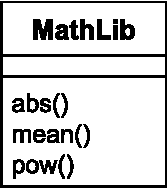
\includegraphics[width=\linewidth]{OriginalClassDiagram}
        \caption{origin}
        \label{fig:origin}
    \end{subfigure}
    \hfill
    \begin{subfigure}[t]{0.2\linewidth}
        \centering
        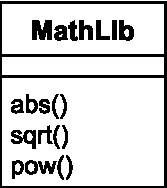
\includegraphics[width=\linewidth]{LeftClassDiagram}
        \caption{left}
        \label{fig:left}
    \end{subfigure}
    \hfill
    \begin{subfigure}[t]{0.2\linewidth}
        \centering
        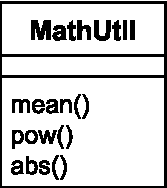
\includegraphics[width=\linewidth]{RightClassDiagram}
        \caption{right}
        \label{fig:right}
    \end{subfigure}
    \hfill
    \label{fig:versions}
    \caption{Different versions of a model.}
\end{figure}
\end{minipage}
\hfill
\begin{minipage}[t]{0.37\linewidth}
\begin{lstlisting}[style=eol,numbersep=0.6pt,caption={The pseudo-formatted CBP of the model in Fig. \ref{fig:origin}.},label=lst:origincbp]
create x type Class
set x.name to "Math" 
create a type Operation
set a.name to "abs" 
create b type Operation
set b.name to "mean" 
create c type Operation
set c.name to "pow" 
add a to x.operations at 0
add b to x.operations at 1
add c to x.operations at 2
\end{lstlisting}
\end{minipage}

\vspace{-5pt}
\section{State-based Model Comparison}
\label{sec:model_comparison}

\vspace{-5pt}
In a collaborative modelling setting, a model can have different versions.
%\dk{Mutliple versions can exist even if a model is developed by a single developer}.
Consider the case where an initial version of a model exists in Version Control System (VCS) server (Fig. \ref{fig:vcs}).
Two modellers, Bob and Alice, checkout the original model (steps 1 and 2) to their local machines and modify it (steps 3 and 4).
Alice then commits her work (original + Alice's changes) to the VCS.
Since there is no newer commit on the VCS, the commit process is straightforward (step 5).
Bob then decides to also commit his work (original + Bob's changes) to the VCS.
However, he needs to merge his work with the current updated version at the VCS since his last checkout.
His machine downloads the latest version from the server (step 6), i.e. Alice's version.
To merge his and Alice's changes, Bob needs to perform model comparison to check their differences, resolve possible conflicts between the models, and then merge them (step 7).
After that, he can push it back to the VCS server.

\begin{figure}[ht]
    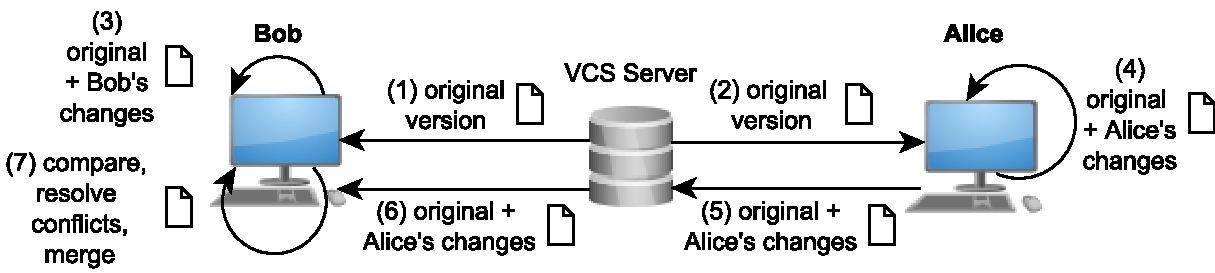
\includegraphics[width=\linewidth]{VCS}
    \caption{A usecase of CBP in a collaborative modelling.}
    \label{fig:vcs}
\end{figure}


In a SBP setting, Bob produces the model in Fig. \ref{fig:left} (the left model), and Alice the model in Fig. \ref{fig:right} (the right model) producing XMI files as shown in List. \ref{lst:leftxmi} and List. \ref{lst:rightxmi} respectively.
Before Bob can merge, he must compare the right model with the left model.
In state-based comparison, comparing models commonly consists of two steps: \emph{matching} and \emph{diffing}.
The matching process establishes matches between the elements of both models, to determine the elements in the left model that correspond to elements in the right model.
Generally, the matching process iterates through all the elements of the models being compared and matches them by their identifiers or through a similarity mechanism  \cite{DBLP:conf/sfm/BroschKLSWW12,emfcompare2018developer}.
%Note that for new and deleted elements the result of the match can be that there is no match.

The diffing process identifies differences between the matched elements \cite{DBLP:conf/sfm/BroschKLSWW12,emfcompare2018developer}.
Differences between the matched elements and all their features is usually done using a Longest Common Subsequence (LCS) algorithm, e.g. \cite{DBLP:journals/algorithmica/Meyers86}.

\vspace{-10pt}
\begin{minipage}[t]{0.49\linewidth} 
\begin{lstlisting}[style=eol,caption={The simplified XMI of the left model in Fig. \ref{fig:left}.},label=lst:leftxmi]
<uml:Class id="x" name="MathLib">
  <operation id="a" name="abs/>
  <operation id="d" name="sqrt"/>
  <operation id="c" name="pow"/>
</uml:Class>
\end{lstlisting}
\end{minipage}
\hfill
\begin{minipage}[t]{0.49\linewidth}
\begin{lstlisting}[style=eol,caption={The simplified XMI of the right model in Fig. \ref{fig:right}.},label=lst:rightxmi]
<uml:Class id="x" name="MathUtil">
  <operation id="b" name="mean"/>
  <operation id="c" name="pow"/>
  <operation id="a" name="abs"/>
</uml:Class>
\end{lstlisting}
\end{minipage}

In our example, the matching process in state-based comparison -- as performed by EMF Compare \cite{emfcompare2018developer} -- iterates through all the elements of both models and matches them using their identifiers. The matching process yields 3 matches: $m_1$ = (\textsf{x}, \textsf{x}), $m_2$ = (\textsf{a}, \textsf{a}), and $m_3$ = (\textsf{c}, \textsf{c}), and 2 unmatched elements, $um_1$ = (\textsf{d}, -) and $um_2$ = (-, \textsf{b}). The diffing process then iterates through all the matches and unmatched elements and uses an LCS algorithm to identify their differences. In the first match, it identifies that the elements \textsf{x} are different in their \textsf{name} and \textsf{operations} features. 

The left \textsf{x}'s \textsf{name} is ``MathLib'' while the other \textsf{x}'s \textsf{name} is ``MathUtil'' (diff $ds_1$). The \textsf{operations} features are different in their contents -- the left \textsf{operations} feature does not contain element \textsf{b} (diff $ds_2$), the left \textsf{operations} feature contains element \textsf{d} 
that does not exist in the right \textsf{operations} (diff $ds_3$), and the indexes of element \textsf{c} are different in both features (diff $ds_4$).

Differences are commonly expressed as a list of changes that must be applied to a target model so that it is made equal to a reference model.
%\dk{We should probably consider different terminology here as the terms ``source'' and ``reference'' are very similar}.
This paper treats the left model as a reference model and the right model as the target model.
This means that differences are expressed as changes applied to the right model so that it equals the left model.
To express differences, we use the following terms: \textsf{LeftContainer}, \textsf{RightContainer}, \textsf{LeftFeature}, \textsf{RightFeature} \textsf{LeftIndex}, \textsf{RightIndex}, \textsf{LeftValue}, \textsf{RightValue}, and \textsf{Kind}. The \textsf{*Container}, \textsf{*Feature}, and \textsf{*Value} are the target element, feature, and value involved in a difference (\textsf{*} symbol can be replaced with \textsf{Left} and {Right}). \textsf{*Index} is the index of a value in a feature. \textsf{Kind} is the type of difference. It can be one of these types: \textsf{CHANGE}, \textsf{ADD}, \textsf{DELETE}, and \textsf{MOVE}. \textsf{CHANGE} means a pair of single-valued features 
%features -- single-valued attributes or non-containment references \dk{Why is containment important?} -- 
have different values. \textsf{ADD} indicates that a value does not exist in the right model thus it requires the addition of the value. \textsf{DELETE} is the opposite
%\dk{``opposite''?} 
of \textsf{ADD}. \textsf{MOVE} indicates that matched elements differ in terms of their containers, containing features, or indexes.
A Container is an element that contains a value. A containing feature is a feature owned by a container in which a value is contained. An index is the position of a value in a containing feature.

Based on these definitions, we can express the result of the diffing process as: $ds_{n}$ = [$LeftContainer_n$, $RightContainer_n$, $LeftFeature_n$, $RightFeature_n$, $LeftIndex_n$, $RightIndex_n$, $LeftValue_n$, $RightValue_n$, $Kind_n$]. Thus, $ds_{1}$ =  [\textsf{x}, \textsf{x}, \textsf{name}, \textsf{name}, 0, 0, ``MathLib'', ``Mathutil'', \textsf{CHANGE}], $ds_{2}$ = [\textsf{x}, \textsf{x}, \textsf{operations}, \textsf{operations}, null, 0, null, \textsf{b}, \textsf{DELETE}], $ds_{3}$ = [\textsf{x}, \textsf{x}, \textsf{operations}, \textsf{operations}, 1, null, \textsf{d}, null, \textsf{ADD}], and $ds_{4}$ = [\textsf{x}, \textsf{x}, \textsf{operations}, \textsf{operations}, 2, 1, \textsf{c}, \textsf{c}, \textsf{MOVE}]. We can use these information to represent the differences visually as depicted in Fig. \ref{fig:xmi_comparison}. Applying these differences as changes to the right model will transform it into the left model.  

\begin{figure}
    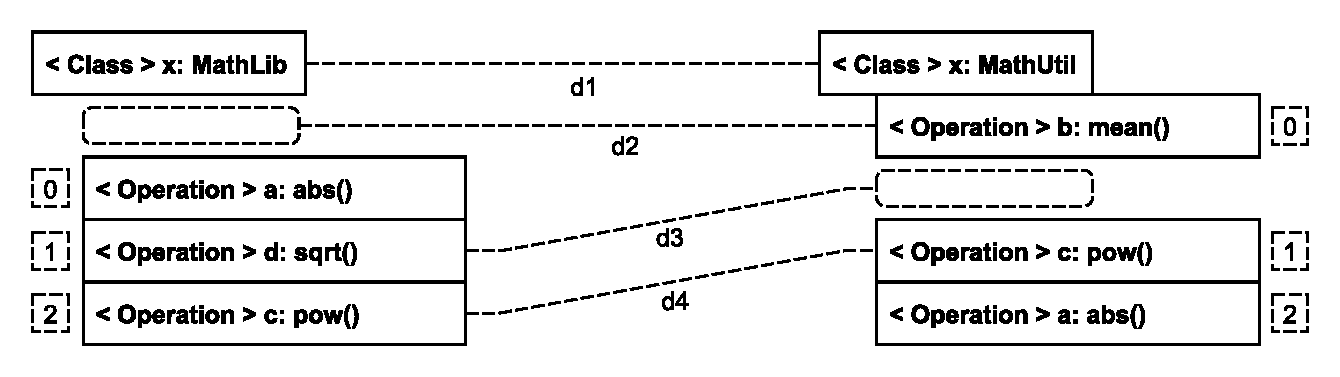
\includegraphics[width=\linewidth]{XmiComparison}
    \caption{A model comparison of the left and right models in Listings \ref{lst:leftxmi} and \ref{lst:rightxmi}.}
    \label{fig:xmi_comparison}
\end{figure}

\section{Change-based Approach for Comparing Models}
\label{sec:change_based_approach_for_comparing_models}

Now lets consider the same example in a CBP setting.
The changes made by Bob and Alice are appended to the their local original CBP producing two different CBP representations as displayed in Listings \ref{lst:leftcbp} and \ref{lst:rightcbp}\footnote{Both CBPs only present the changes after the last line of the original version (start from line 12).} -- capturing different courses of modification made by both modellers.
Then the example is the same with Alice committing her changes and Bob wanting to merge Alice's work with his. 


\begin{minipage}[t]{0.49\linewidth}    
\begin{lstlisting}[firstnumber=12,style=eol,caption={The appended changes made by Bob to produce the model in Fig. \ref{fig:left}  (left version).},label=lst:leftcbp]
set x.name from "Math" to "MathLib"
create d type Operation
set d.name to "sqrt"
add d to x.operations at 1
remove b in x.operations at 2
delete b
\end{lstlisting}
\end{minipage}
\hfill
\begin{minipage}[t]{0.49\linewidth}
\begin{lstlisting}[firstnumber=13,style=eol,caption={The appended changes made by Alice to produce the model in Fig. \ref{fig:right} (right version).},label=lst:rightcbp]
move a in x.operations from 0 to 2
set x.name from "Math" to "MathUtil"
\end{lstlisting}
\end{minipage}

%Since both modellers work using CBP, we can exploit the representation to improve the previous model comparison.
%For example, we do not need to visit, match, and differentiate both \textsf{c} elements in the running example as they are not affected by the recent changes in both CBPs; only the affected features by the recent changes to be compared -- not all features. 
In CBP, comparison has three phases: event loading, element tree construction, and diff computation.
Further, comparison is not performed over all the elements of the model; instead, we only need to compare the last set of changes from the source and reference model.
The last set of changes can be easily identified by finding their last common change.
A simplified class diagram of our approach's implementation\footnote{The source can be found at \url{https://github.com/epsilonlabs/emf-cbp}.} is depicted in Fig. \ref{fig:approach_class_diagram}. 
Next, we describe the three phases in detail.

\begin{figure}
    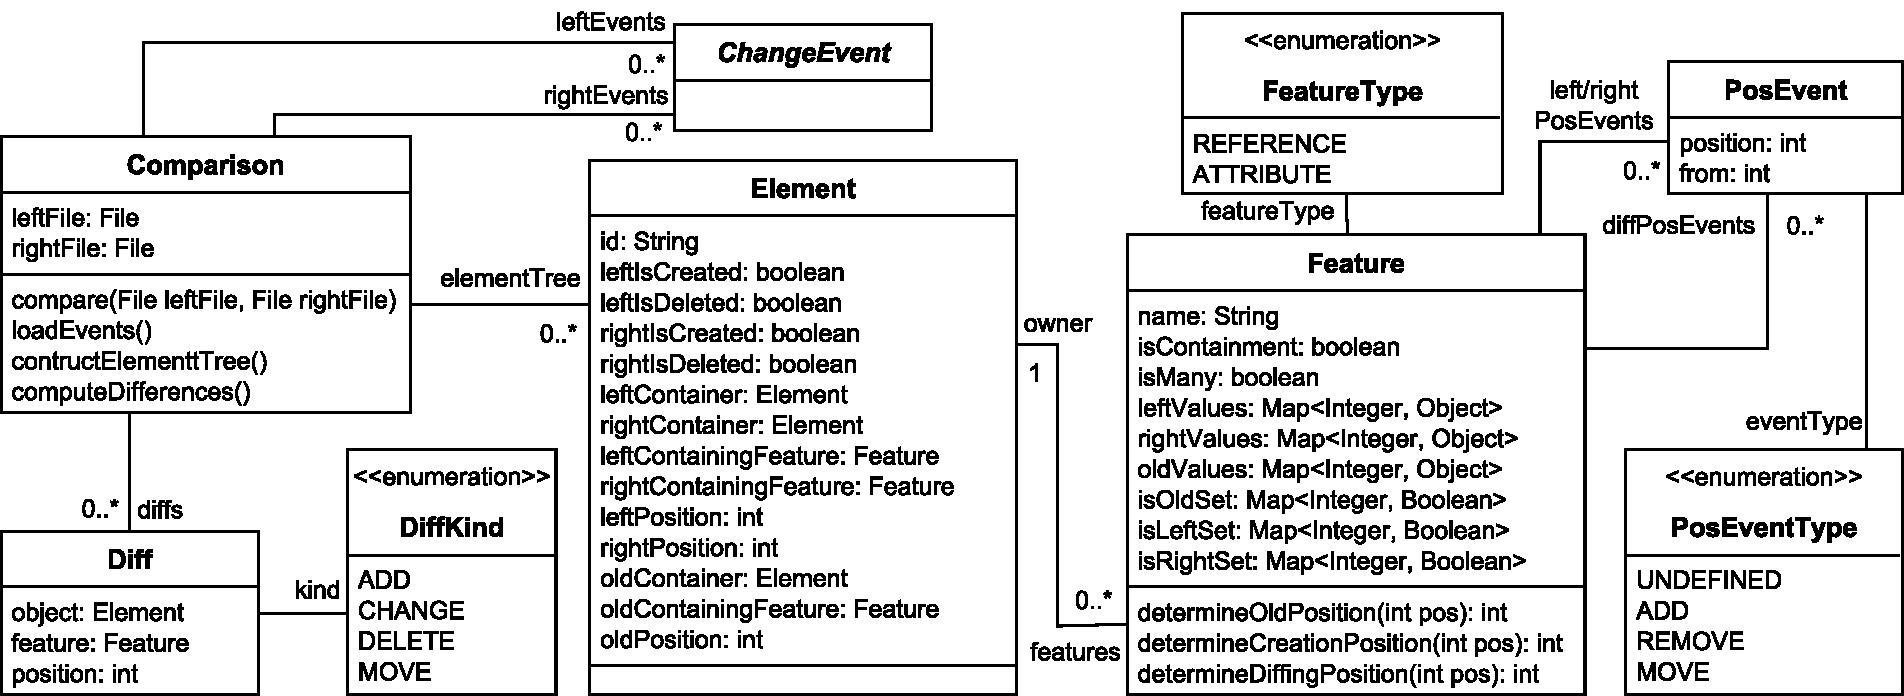
\includegraphics[width=\linewidth]{TreeClassDiagram}
    \caption{A class diagram showing the core components of the change-based approach to speed up model comparison.}
    \label{fig:approach_class_diagram}
\end{figure}


\subsection{Event Loading}
\label{sec:event_loading}
In the event loading phase, our implementation loads change events recorded in two CBP files into memory.
The most important aspect of this phase is the partial loading as only lines starting from the position where the two files are different are loaded.
Thus, not the whole model needs to be traversed and loaded.
In this case, lines 1-11 in List. \ref{lst:origincbp} are skipped.

Only lines starting from line 12 in Listings \ref{lst:leftcbp} and \ref{lst:rightcbp} are loaded, yielding two partial -- left and right -- change-event models. 

\subsection{Element Tree}
\label{sec:tree_construction}
An element tree is a representation of the changes of model elements in the source and reference models.
It contains detailed information about elements and their properties.

It contains similar information to that captured in change lists in SBP, but also provides more information about the changes.
For example, the element tree can keep track of a feature's old value and element/value's indexes inside multi-valued properties. 
%The latter reduces false-positives when detecting MOVE changes. 

%These specific features are useful to determine differences in the diff computation phase (Section \ref{sec:diff_computation}).
The element tree only contains the partial states -- not whole -- of affected elements of original, left, and right models as depicted in Figures \ref{fig:left_element_tree_diagram} and \ref{fig:right_element_tree_diagram}.

To better understand the construction of an element tree from change events, we use the following running example using both change events in the Listings \ref{lst:leftcbp} and \ref{lst:rightcbp}. We start from the left change events. 


\begin{wrapfigure}[38]{r}{0.5\textwidth}
    \vspace{-20pt}
    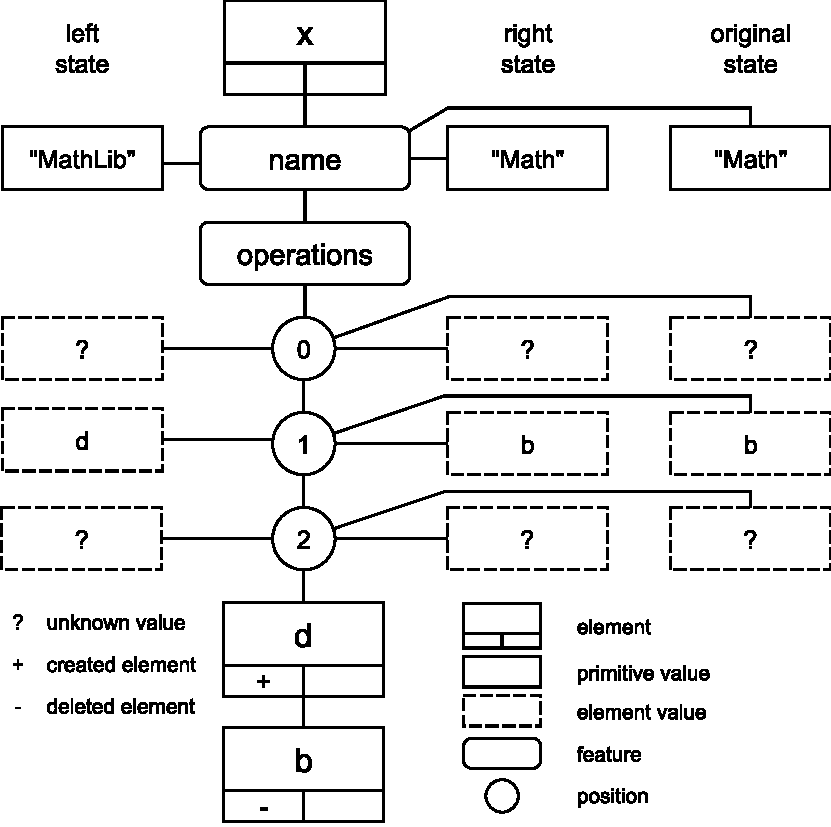
\includegraphics[width=\linewidth]{LeftElementTreeDiagram}
    \caption{The \textsf{elementTree} after processing all left change events.}
    \label{fig:left_element_tree_diagram}
    \vspace{1em}
    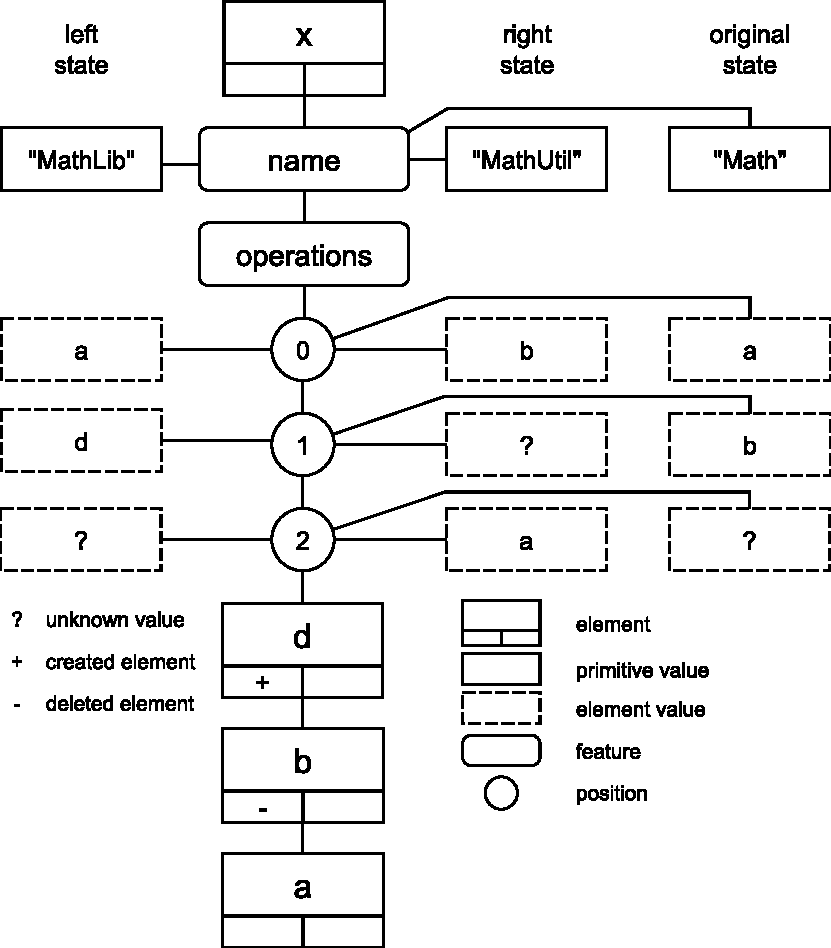
\includegraphics[width=\linewidth]{RightElementTreeDiagram}
    \caption{The \textsf{elementTree} after processing all left and right change events.}
    \label{fig:right_element_tree_diagram}
\end{wrapfigure}

\subsubsection{Left Side}\label{sec:left_side}
%In List. \ref{lst:leftcbp}, 

From the first event [\texttt{\small \textbf{set} x.name \textbf{from} "Math" \textbf{to} "MathLib"}] at line 12, we can identify that an element with id \textsf{x} that exists from the original model. It has a feature \textsf{name} with a value ``Math'' in the original model that has been changed to ``MathLib'' in the left model. Since the element \textsf{x} has not existed in the \textsf{elementThree}, we create its instance of \textsf{Element} and also its feature \textsf{name}. We set the value of the feature \textsf{name} to ``MathLib'' and also set it to ``Math'' in the partial state of the original model -- it has not been set before. As this feature on the right side also has not been set, we set it to ``Math'' as well. 
%Once a feature in the original state has been set, it cannot be overridden -- using the flag \textsf{isOldSet} in class \textsf{Feature} in Fig. \ref{fig:approach_class_diagram}. 

At line 13, in the event [\texttt{\small \textbf{create} d \textbf{type} Operation}], we can identify that there an element with id \textsf{d} has been created. We also update the \textsf{elementTree} to include this element and set the element's flag \textsf{leftIsCreated} to \textsf{true}. In the event [\texttt{\small \textbf{set} d.name \textbf{to} "sqrt"}] at line 14, we can identify that element \textsf{d}'s feature \textsf{name} has been set to ``sqrt''. Thus, we update the \textsf{d}'s feature \textsf{name} in the \textsf{elementTree}. From the event [\texttt{\small \textbf{add} d \textbf{to} x.operations \textbf{at} 1}] at line 15, we can deduce that element \textsf{d} is added to index 1 in the element \textsf{x}'s feature \textsf{operations}. Thus, we assign \textsf{d} to element \textsf{x}'s feature \textsf{operations} at index 1 in the \textsf{elementTree}. As \textsf{d} is a new element that only exists in the left model, we do not update changes of this element to the original and right models. 

From the event [\texttt{\small \textbf{remove} b \textbf{in} x.operations \textbf{at} 2}] at line 16, we can identify that there is element \textsf{b} in the original model, but it is deleted in the left model. The index of element \textsf{b} in the original model can be calculated back through the previous change events that have been applied to its feature. Since the previous event is adding element \textsf{d} to index 1 and the index of \textsf{b} is at 2 at the time it is removed, we can deduce that before element \textsf{d} is added, the index of element \textsf{b} is at 1 and is shifted to 2 because of the addition of element \textsf{d}.  Therefore, we can conclude that the original index of element \textsf{b} is at 1. Thus, we update the original state of the \textsf{elementTree} by adding element \textsf{b} into the element \textsf{x}'s feature \textsf{operations} at index 1.  

We perform the same procedure to also add element \textsf{b} to the right state of the \textsf{elementTree}. However, since there is no change event has been applied to right side of element \textsf{x}'s feature \textsf{operations}, the calculation of element \textsf{b}'s index should return the same value as in the original state (line 13, Alg. \ref{alg:element_tree}), and thus element \textsf{b} has the same index as in the original state. It is important to notice, in this step, the flag \textsf{isRightSet} (class \textsf{Feature}, Fig. \ref{fig:approach_class_diagram}) is not set to \textsf{true} since we want the value to be able to be overridden during processing of the right change events. The last event [\texttt{\small \textbf{delete} b}], removes the element \textsf{b} from the left model. Hence, we set the flag \textsf{leftIsDeleted} of element \textsf{a} to \textsf{true}.

Fig. \ref{fig:left_element_tree_diagram} illustrates the state of the \textsf{elementTree} after all left change events have been processed. As can be seen, the \textsf{elementThree} exhibits the partial states of the original, left, and right models at once. 

\subsubsection{Right Side}\label{sec:right_side}  From the first event [\texttt{\small \textbf{move} a \textbf{in} x.operations \textbf{from} 0 \textbf{to} 2}] at line 12, we can infer that in the right model there is an element with id \textsf{a} positioned at index 2 in the element \textsf{x}'s feature \textsf{operations}. Thus, element \textsf{a} -- an instance of class \textsf{Element} in \ref{fig:approach_class_diagram} -- is added to the \textsf{elementTree} and positioned at index 2 of the element \textsf{x}'s feature \textsf{operations}. Since the event is a \textsf{move} type and the new index is larger than its previous index, elements that are between its previous and new indexes are shifted one place down. As element \textsf{b} has already existed in the same feature (the element was added during the process of the left change events) and its index is between element \textsf{a}'s movement, the index of element \textsf{b} is shifted down from 1 to 0. 

Also since the event's type is \textsf{move} and its previous index is 0 and it is the first event that changes the index of element \textsf{a}, these conditions imply that element \textsf{a} in original model is positioned at index 0 in the element \textsf{x}'s feature \textsf{operations}. Therefore, we add the element \textsf{a} to  the element \textsf{x}'s feature \textsf{operations} in the original state of the \textsf{elementTree}. Since the index 0 in the element \textsf{x}'s feature \textsf{operations} has not been set, we also add element \textsf{a} to that index in the right state of the \textsf{elementTree}. From the last event [\texttt{\small \textbf{set} a.name \textbf{from} "Math" \textbf{to} "MathUtil"}] at line 13, we can infer that in the right model the value of element \textsf{a}'s feature \textsf{name} is ``MathUtil'' in the right model. Hence, we set the feature \textsf{name} to ``MathUtil'' in the right state. We do apply this operation to the original and left states as they have been set before. Fig. \ref{fig:right_element_tree_diagram} exhibits the state of the \textsf{elementTree} after both side change events have been processed.

\begin{figure}
    \centering
    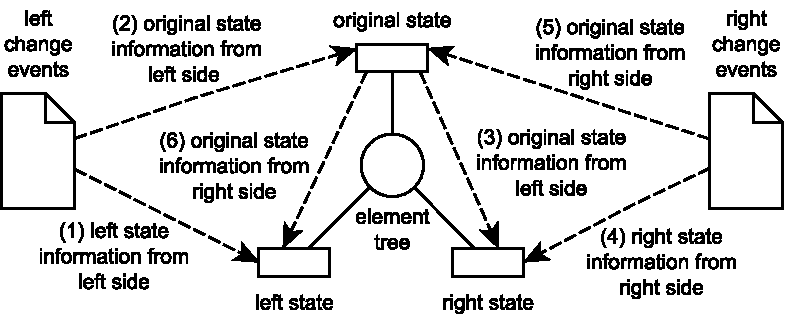
\includegraphics[width=0.7\linewidth]{TreeConstruction}
    \caption{Steps in Element Tree construction.}
    \label{fig:tree_construction}
\end{figure} 

The construction of the \textsf{elementTree} that we have just explained follows the steps shown in Fig. \ref{fig:tree_construction}. First, the partial left state $S_{L}$ of a left model in the \textsf{elementTree} is constructed based on the information retrieved from the left change events (step 1). We denote this information as $I_{LL}$. We can also construct the partial original state $S_{O}$ of the original model using the information related to the original state contained in the left change events $I_{OL}$ (step 2). The information $I_{OL}$ facilitates us to construct the initial partial right state $S_{R}$ of the right model before updated by the right change events (step 3). Similarly, using the information from the right change events $I_{RR}$, we update the partial right state $S_{R}$ that has been initialised before using the information $I_{OL}$ (step 4), implying that $I_{OL} \cup I_{RR} \rightarrow S_{R}$. Also, information related to the state of the original model from the right change events is used to update the original state $I_{OR}$ (step 5). Thus, we have a more representative partial state of the original model using information from both sides, $I_{OL} \cup I_{OR} \rightarrow S_{O}$. The $I_{OR}$ is also used to update the left state to have a more representative partial state of the left model (step 6). Thus,  $I_{LL} \cup I_{OR} \rightarrow S_{L}$.  


\IncMargin{1.5em}
\begin{algorithm}[H]
    \begin{footnotesize}
        \SetKwInOut{Input}{input}
        \SetKwInOut{Output}{output}
        \Input{a list of ChangeEvent $events$}
        \Input{an enumeration of Side $side$}
        \Input{an instance of ElementTree $elementTree$}
        \Output{an instance of ElementTree $elementTree$}
        \SetKwBlock{Beginn}{beginn}{ende}
        \Begin{
            \ForEach{$event$ in $events$}{
                $targetElement$ $\leftarrow$ getOrCreateNewTargetElement($event$, $elementTree$)\;
                $feature$ $\leftarrow$ getOrCreateNewFeature($event$, $targetElement$)\;
                $value$ $\leftarrow$ getValue($event$)\;
                $previousValue$ $\leftarrow$ getPreviousValue($event$)\;
                $index$ $\leftarrow$ getIndex($event$)\;
                $previousIndex$ $\leftarrow$ getPreviousIndex($event$)\;
                $featureEventList$ $\leftarrow$ getFeatureEventList($feature$, $side$)\;
                
                \BlankLine
                \tcp{put all values to their proper indexes}
                updateTree($targetElement$, $feature$, $value$, $index$, $side$)\;
                $oldIndexes$ $\leftarrow$ calculateOldIndex($featureEventList$, $previousIndex$, $side$)\;
                \If{\Not isCreated($value$, $side$) \And \Not isOldValueSet($feature$, $previousValue$, $previousIndex$, $side$)} {
                    setOldValue($feature$, $previousValue$, $oldIndex$, $side$)\;
                    $oppositeFeatureEventList$ $\leftarrow$ getOppositeFeatureEventList($feature$, $side$)\;
                    $oppositeIndex$ $\leftarrow$ calculateOppositeIndex($oppositeFeatureEventList$, $oldIndex$, $side$)\;
                    \If{\Not isDeleted($value$, $side$) \And \Not isOppositeSideValueSet($feature$, $value$, $oppositeIndex$, $side$)} {
                        setOppositeSideValue($feature$, $value$, $oppositeIndex$, $side$)\;
                    }
                }   
                
                addEventToFeatureEventList($event$, $featureEventList$)\;
                
            }
            \Return{$elementTree$}\;
        }
    \end{footnotesize}
    \caption{Algorithm to construct an element tree from events.}
    \label{alg:element_tree}
\end{algorithm}
\DecMargin{1.5em}

The Alg. \ref{alg:element_tree} is an algorithmic view of the steps presented in Fig. \ref{fig:tree_construction}. Basically, it iterates through all a model's change events and uses the information contained in the change events to construct the relevant partial state. The selection of side, left or right change events, that is executed first depends on the \textsf{Side} enumeration value -- \textsf{left} or \textsf{right} -- passed through the parameter \textsf{side} (the second input parameter). In our implementation, we process the left side first. The algorithm also receives an input of the change events \textsf{events} that are to be iterated and the element tree \textsf{elementTree} that has been instantiated before, and then return the \textsf{elementTree} as output after updating it.

For each \textsf{event} in the \textsf{events}, we collect information needed to build up the \textsf{elementTree}  (lines 3-9), such as \textsf{targetElement}, \textsf{feature}, \textsf{value}, \textsf{previousValue}, \textsf{index}, and \textsf{previousIndex}. The \textsf{targetElement} is the element modified by a change event (e.g. \textsf{x} and \textsf{d} in List. \ref{lst:leftcbp}). This \textsf{targetElement} -- an instance of class Element in Fig. \ref{fig:approach_class_diagram} -- is retrieved from the \textsf{elementTree} if it already exists. Otherwise, a new element is created and added to the \textsf{elementTree} (line 3). In this step also we set the flags \textsf{*IsCreated} and \textsf{*IsDeleted} of the element in Fig. \ref{fig:approach_class_diagram}. For example, if the type of the event is \textsf{create} then \textsf{*IsCreated} is set to \textsf{true}. The \textsf{feature} -- an instance of class Feature in Fig. \ref{fig:approach_class_diagram} -- represents the target element's feature (e.g. \textsf{name} and \textsf{operations} in List. \ref{lst:leftcbp}) modified by a change event. It is  retrieved from the \textsf{targetElement}'s feature list, and a new one is created and added to the \textsf{targetElement}'s feature list if it has not existed yet (line 5). 

The \textsf{value} is the value assigned to the feature in a change event (line 5, Alg. \ref{alg:element_tree}). The \textsf{value} can be the type of \textsf{Element} (e.g. elements \textsf{b} and  \textsf{d}, lines 17-18, List. \ref{lst:leftcbp}) or primitive (e.g. the String ``MathLib'' at line 14 in the List. \ref{lst:leftcbp}). The \textsf{previousValue} represents the previous value of the modified feature (line 6, Alg. \ref{alg:element_tree}). The \textsf{previousValue} is not defined if no previous value has been assigned. For \textsf{value} and \textsf{previousValue} with type \textsf{Element}, the elements that they represent are retrieved from the \textsf{elementTree}, and if they do not exists, new instances are created. If the type is primitive, the value is treated as it is. Not every change event has \textsf{value}, particularly event with type \textsf{add} or \textsf{delete} as it only modifies a target element not the element's feature.

The \textsf{index} is the index assigned by a change event to a value in a feature, while \textsf{previousIndex} is the previous index of the value (lines 7-8, Alg. \ref{alg:element_tree}). In one change event, we can get both \textsf{index} and \textsf{previousIndex} or only one of them depends on the type of the change event. For example, we can only obtain that the \textsf{index} of \textsf{d} is 1 (line 17 in in the List. \ref{lst:leftcbp}) as the change event type is \textsf{add}. In a \textsf{remove} change event, we can only get the \textsf{previousIndex} of \textsf{b}, that is 2 (line 17 in in the List. \ref{lst:leftcbp}), as the element does not exist anymore in the left model. We can obtain both of them only in a \textsf{move} change event as an element is moved from a previous index to a new one (line 14 in in the List. \ref{lst:rightcbp}). For a single-valued feature, the \textsf{index} and \textsf{previousIndex} are always 0 as the feature can only contain a single value. 

At line 9, we retrieve the \textsf{featureEventList} from the \textsf{feature} to be added later with the current \textsf{event} (line 19). The \textsf{featureEventList} is a list -- a history -- of change events that have been processed that are specific to the \textsf{feature} on the selected \textsf{side}. Using the obtained \textsf{targetElement}, \textsf{feature}, \textsf{value}, and \textsf{index}, the process then updates the state of the \textsf{elementTree} on the selected \textsf{side} (line 10). After that, it calculates back the original index of a value using the \textsf{featureEventList} and \textsf{previousIndex} (line 11). If the value at \textsf{oldIndex} in the \textsf{feature} has not been set, then the algorithm sets the \textsf{feature} with the \textsf{previousValue} at the \textsf{oldIndex} in the partial state of the original model (lines 12-13). At lines 14-18, the algorithm also does the same thing to the opposite side -- if the current \textsf{side} is \textsf{left} then it is \textsf{right}.  

\subsection{Diff Computation}
\label{sec:diff_computation}

Using the \textsf{elementTree} presented in Fig. \ref{fig:right_element_tree_diagram}, we can determine the difference between the left and right models without having to compare all their elements and features. After the \textsf{elementTree} has been constructed, we iterate through elements and features of the \textsf{elementTree} and use the flags, containers, containing features, and indexes on both sides of each element and value to identify differences between both left and right models. We follow the steps in Alg. \ref{alg:diff_calculation}. The algorithm visits each element and every index of each feature (lines 3-5). At every index, it retrieves the \textsf{leftValue} and \textsf{rightValue} (lines 5-7), passing these, together with the \textsf{element}, \textsf{feature}, and \textsf{index} to a function \textsf{identifyDiffUsingRules} (line 8). The function identifies differences using a set of pre-defined rules which determines differences \textsf{diffs} based on the states of flags of an element, flags and attributes of the element's feature, values of the feature, and indexes of the values. The obtained \textsf{diffs} are then added to the overall list of differences \textsf{diffList} which is output (line 8-9, 13). 

\IncMargin{1.5em}
\begin{algorithm}[H]
    \begin{footnotesize}
        \SetKwInOut{Input}{input}
        \SetKwInOut{Output}{output}
        \Input{an instance of ElementTree $elementTree$}
        \Begin{
            $diffList$ $\leftarrow$  DiffList()\;
            \ForEach{$element$ \In $elementTree$}{
                \ForEach{$feature$ \In getFeatures($element$)}{
                    \ForEach{$index$ \In getIndexes($feature$)}{
                        $leftValue$ $\leftarrow$ getLeftValue($feature$, $index$)\;
                        $rightValue$ $\leftarrow$ getRightValue($feature$, $index$)\;
                        \BlankLine
                        \tcp{rules starts from here}
                        $diffs$ $\leftarrow$ identifyDiffUsingRules($element$, $feature$, $leftValue$, $rightValue$, $index$)\;
                        addToDiffList($diffs$,$diffList$)\;
                    }
                }
            }
            \Return{$diffList$}\;
        }
    \end{footnotesize}
    \caption{Algorithm to determine differences.}
    \label{alg:diff_calculation}
\end{algorithm}
\DecMargin{1.5em}

The first rule (Rule 1) in Alg. \ref{alg:diff_rules} is to identify a change of value of a single-valued attribute. A feature has to be of type of \textsf{attribute}, both side values have to be different, and the element should have not been created or deleted in both models. The second rule (Rule 2) is to identify that an element is in different location in both models. The element must not have been deleted and must exist from the the previous version -- the original model. Also, its containers, containing features, or indexes of the element have to be different on both sides.

We illustrate the principles and use of rules by discussing the rules used to identify differences in the running example, which can be found in Alg. \ref{alg:diff_rules}. The algorithm is the breakdown of the function \textsf{identifyDiffUsingRules} in Alg. \ref{alg:diff_calculation}. As previously stated, it is important to remember that we use the left model as a reference which means the differences are presented as changes that transform the right model to become equal to the left model. 

\IncMargin{1.5em}
\begin{algorithm}[H]
    \begin{footnotesize}
        \SetKwInOut{Input}{input}
        \SetKwInOut{Output}{output}
        \Input{an Element $element$, a Feature $feature$, a variable $leftValue$, a variable $rightValue$, an Integer $index$}
        \Output{a List of Diff $diffs$}
        $diffs$ $\leftarrow$ createDiffList()\;
        \tcp{...}
        \tcp{Rule 1: a rule to determine a change of a single-valued attribute}
        \If{getType($feature$) \Is Attribute \And isSingleValued($feature$) \And leftValue <> rightValue \And \Not leftIsCreated($element$) \And \Not leftIsDeleted($element$) \And \Not  rightIsCreated($element$) \And \Not rightIsDeleted($element$)}{
            $diff$ $\leftarrow$ createNewDiff($element$, $element$, $feature$, $feature$, $index$, $index$, $leftValue$, $rightValue$, DifferenceType.CHANGE)\;
            addDiffToDiffList($diff$, $diffs$)\;
        } 
        \tcp{Rule 2: one of rules to determine movement of an element}
        \If{getType($feature$) \Is Containment \And \Not leftIsCreated($leftValue$) \And \Not leftIsDeleted($leftValue$) \And \Not rightIsCreated($leftValue$) \And \Not rightIsDeleted($leftValue$) \And (getLeftContainer($leftValue$) <> getRightContainer($leftValue$) \Or getLeftFeature($leftValue$) <> getRightFeature($leftValue$) \Or getLeftIndex($leftValue$) <> getRightIndex($leftValue$))}{
            $diff$ $\leftarrow$ createNewDiff(getLeftContainer($leftValue$), getRightContainer($leftValue$), getLeftFeature($leftValue$), getRightFeature($leftValue$), getLeftIndex($leftValue$), getRightIndex($leftValue$), leftValue, leftValue, DifferenceType.MOVE)\;
            addDiffToDiffList($diff$, $diffs$)\;
        }
        \tcp{Rule 3: one of rules to determine deletion of an element}
        \If{getType($feature$) \Is Containment \And \Not leftIsCreated($rightValue$) \And leftIsDeleted($rightValue$) \And \Not rightIsCreated($rightValue$) \And \Not rightIsDeleted($rightValue$) }{
             createNewDiff(getLeftContainer($rightValue$), getRightContainer($rightValue$), getLeftFeature($rightValue$), getRightFeature($rightValue$), getLeftIndex($rightValue$), getRightIndex(), rightValue, null, DifferenceType.DELETE)\;
            addDiffToDiffList($diff$, $diffs$)\;
       }
        \tcp{Rule 4: one of rules to determine addition of an element}
        \If{getType($feature$) \Is Containment \And leftIsCreated($leftValue$)  \And \Not leftIsDeleted($leftValue$) \And \Not rightIsCreated($leftValue$) \And \Not rightIsDeleted($leftValue$)}{
            $diff$ $\leftarrow$ createNewDiff(getLeftContainer($leftValue$), getRightContainer($leftValue$), getLeftFeature($leftValue$), getRightFeature($leftValue$), getLeftIndex($leftValue$), getRightIndex($leftValue$), null, rightValue, DifferenceType.ADD)\;
            addDiffToDiffList($diff$, $diffs$)\;
        }
        \tcp{...}
        \Return{$diffs$}
    \end{footnotesize}
    \caption{Some rules to determine differences.}
    \label{alg:diff_rules}
\end{algorithm}
\DecMargin{1.5em}

The third rule (Rule 3) is to identify the deletion of an element. If an element in the left model is not created but exists in the model, it means that the element has been there from the previous version -- the original model. This also means that the element also exists in the right model, unless it has been deleted. Thus, in order to make the right model equals to the left model, the element has to be deleted also in the right model. The fourth rule (Rule 4) is to identify the need for an addition of an element. If an element is created in the left model and has not been deleted, it means that the element should be added also to the right model to make both models equal.

In the running example, when the iteration of the \textsf{elementTree} (Fig. \ref{fig:right_element_tree_diagram}) returns feature \textsf{name}, the type of the feature is a single-valued attribute and both sides of the feature are different in their values, this means that the condition of the first rule is met. Thus, we can conclude that in order to make the left value of the feature equal to the right value, we must override the value ``MathUtil'' with ``MathLib''; the type of this difference is \textsf{CHANGE}. When the iteration is at index 0 in the element \textsf{x}'s feature \textsf{operations}, we have two values: the \textsf{leftValue} is element \textsf{a}, and the \textsf{rightValue} is element \textsf{b}. At \textsf{a} it exists on both sides -- all flags \textsf{*Created} and \textsf{*Deleted} are false --, and it also has different index, at 0 in the left state and 2 in the right state. This condition meets the second rule. Thus, we can conclude that in order to make the index of element \textsf{a} in the right model equals its index in the left model, element \textsf{a} should be moved from index 2 to 0. Thus, the type of this difference is \textsf{MOVE}. 

Element \textsf{b} used to exist but has been deleted from the left model (flags \textsf{leftIsCreated} = false, \textsf{leftIsDeleted} = true); it still exists in the right state (flags \textsf{rightIsCreated} = false, \textsf{rightIsDeleted} = false). This condition satisfies the third rule. Therefore, the element \textsf{b} should be deleted from the right model; the type of this difference is \textsf{DELETE}. We can get only one value when the iteration is at index 1 in the element \textsf{x}'s feature \textsf{operations}; the \textsf{leftValue} is element \textsf{d}, but the \textsf{rightValue} is unidentified. Thus we only process the \textsf{leftValue}. Element \textsf{d} is only created in the left model (flags \textsf{leftIsCreated} = true, \textsf{leftIsDeleted} = false, \textsf{rightIsCreated} = false, \textsf{rightIsDeleted} = false). This condition meets the fourth rule. Thus, to make element \textsf{d} also exist in the right state, we must add it into element \textsf{x}'s feature \textsf{operations} at index 1. Therefore, the type of this difference is \textsf{ADD}. At index 2, the element \textsf{a} is skipped because it has been processed already. 

Similar to the state-based approach in Section \ref{sec:model_comparison}, we express identified differences as $dc_{n}$ = [$LeftContainer_n$, $RightContainer_n$, $LeftFeature_n$, $RightFeature_n$, $LeftIndex_n$, $RightIndex_n$, $LeftValue_n$, $RightValue_n$, $Kind_n$]. Thus, $dc_{1}$ =  [\textsf{x}, \textsf{x}, \textsf{name}, \textsf{name}, 0, 0, ``MathLib'', ``Mathutil'', \textsf{CHANGE}], $dc_{2}$ = [\textsf{x}, \textsf{x}, \textsf{operations}, \textsf{operations}, ?, 0, ?, \textsf{b}, \textsf{DELETE}], $dc_{3}$ = [\textsf{x}, \textsf{x}, \textsf{operations}, \textsf{operations}, 1, ?, \textsf{d}, ?, \textsf{ADD}], and $dc_{4}$ = [\textsf{x}, \textsf{x}, \textsf{operations}, \textsf{operations}, 0, 2, \textsf{a}, \textsf{a}, \textsf{MOVE}]. This change-based approach might produce differences that are different from differences that the state-based approach produces. This can be seen between by comparing $ds_{4}$ and $dc_{4}$ ($ds_{4}$ $\neq$ $dc_{4}$, [\textsf{x}, \textsf{x}, \textsf{operations}, \textsf{operations}, 2, 1, \textsf{c}, \textsf{c}, \textsf{MOVE}] $\neq$ [\textsf{x}, \textsf{x}, \textsf{operations}, \textsf{operations}, 0, 2, \textsf{a}, \textsf{a}, \textsf{MOVE}]). In the state-based approach, element \textsf{c} has a \textsf{MOVE} difference -- it has different index ($ds_{4}$), while in the change-based approach, this difference is attributed to element \textsf{a} ($dc_{4}$). However, in both approaches, if we resolve their differences by performing all-left-to-right merging  -- making the right model equal to the left model, both approaches produce two models that are equivalent. In this way, we can check the correctness of the identified differences produced by the change-based approach.

\section{Evaluation}
\label{sec:evaluation}
In this section, we present the method that we employed to evaluate our change-based comparison approach and discuss the results. We also present the limitation and validity of the evaluation.
\subsection{Method}
\label{sec:method}
In order to assess the performance of the change-based approach in comparing models, we have evaluated it against the traditional state-based approach. We choose EMF Compare \cite{emfcompare2018developer,eclipse2017compare} as the tool to perform the state-based comparison since, it is a mature and commonly used tool to compare EMF-based models. Since we could not find any existing large models persisted in change-based format, the dataset for our experiments is reverse-engineered from a large model from the Epsilon project \cite{eclipse2018epsilongit,eclipse2017epsilon}. This model conforms to the Java metamodel \cite{eclipse2018modiscojava} and consists of more than 1.6 million elements with a size of 224 MBs persisted in XMI format. 

We cloned the original model to produce two new left and right -- models and perform operations (\textsf{add}, \textsf{remove}, \textsf{move}, \textsf{set} with random elements, features, indexes, and values) on both models to create differences. We made 1.1 million artificial changes to each model, generating over 1.1 million events (one operation can generate more than one event, e.g. a \textsf{move} between features generates \textsf{remove} and \textsf{add} events). Events generated by the changes were persisted in change-based format (to be used later in change-based model comparison). After every 50 thousand changes, we made a measurement point. We persisted the last state of the models in state-based format (to be used later in state-based model comparison) and then performed the change-based and state-based model comparison and measured their comparison time and memory footprint. We made 22 measurement points to capture their trends in one batch of measurement. 

We performed 5 batches of measurement. In the first batch, the ratio of occurrence between \textsf{add}, \textsf{remove}, \textsf{move}, and \textsf{set} operations is set to 1:1:20:40 intuitively in assumption that in a mature model modification -- \textsf{move} and \textsf{set} -- occurs more frequent than addition and deletion. Since we wanted the change of total elements did not affect our measurement, the number of total elements should be kept constant. For example, it is difficult to tell an increase of time in comparison is caused by an increase in number of elements or number of change events. One way to do this was by not executing \textsf{add} and \textsf{remove} operations. However, excluding both operations made measurement less representative. Thus, we still included both operations but made their probabilities equal so that the number of total elements can be constant. To support the result of the first batch, in the rest of the batches, we only performed homogeneous type operations -- isolated from other types -- per batch (e.g. add-only, move-only operations). In the end, we obtained 5 results of the batches: mixed, add-only, remove-only, move-only, and set-only measurement results.

For the change-based approach, the comparison time is the duration required for loading change events, constructing an element tree, and identifying differences. The memory footprint is the space used to hold the change events, element tree, and differences in memory. For the state-based approach, the comparison time is the time span required for matching elements and identifying differences, and the memory footprint is the space required to hold the matches and differences in memory. All measurements were performed on the same machine.

Since the change-based and state-based approaches can produce different differences, in order to evaluate the correctness of the change-based approach, we reconciled all the differences by performing all-left-to-right merging -- making the right model identical to the left model -- based on the identified differences. If the all-left-to-right merging of change-based approach produces a model that is identical to the model produced by the all-left-to-right merging of the state-based approach then it can be said that differences identified by the change-based approach are correct. We performed this correctness checking at every measurement point.

\begin{wrapfigure}[38]{r}{0.5\textwidth}
    \vspace{-26pt}
    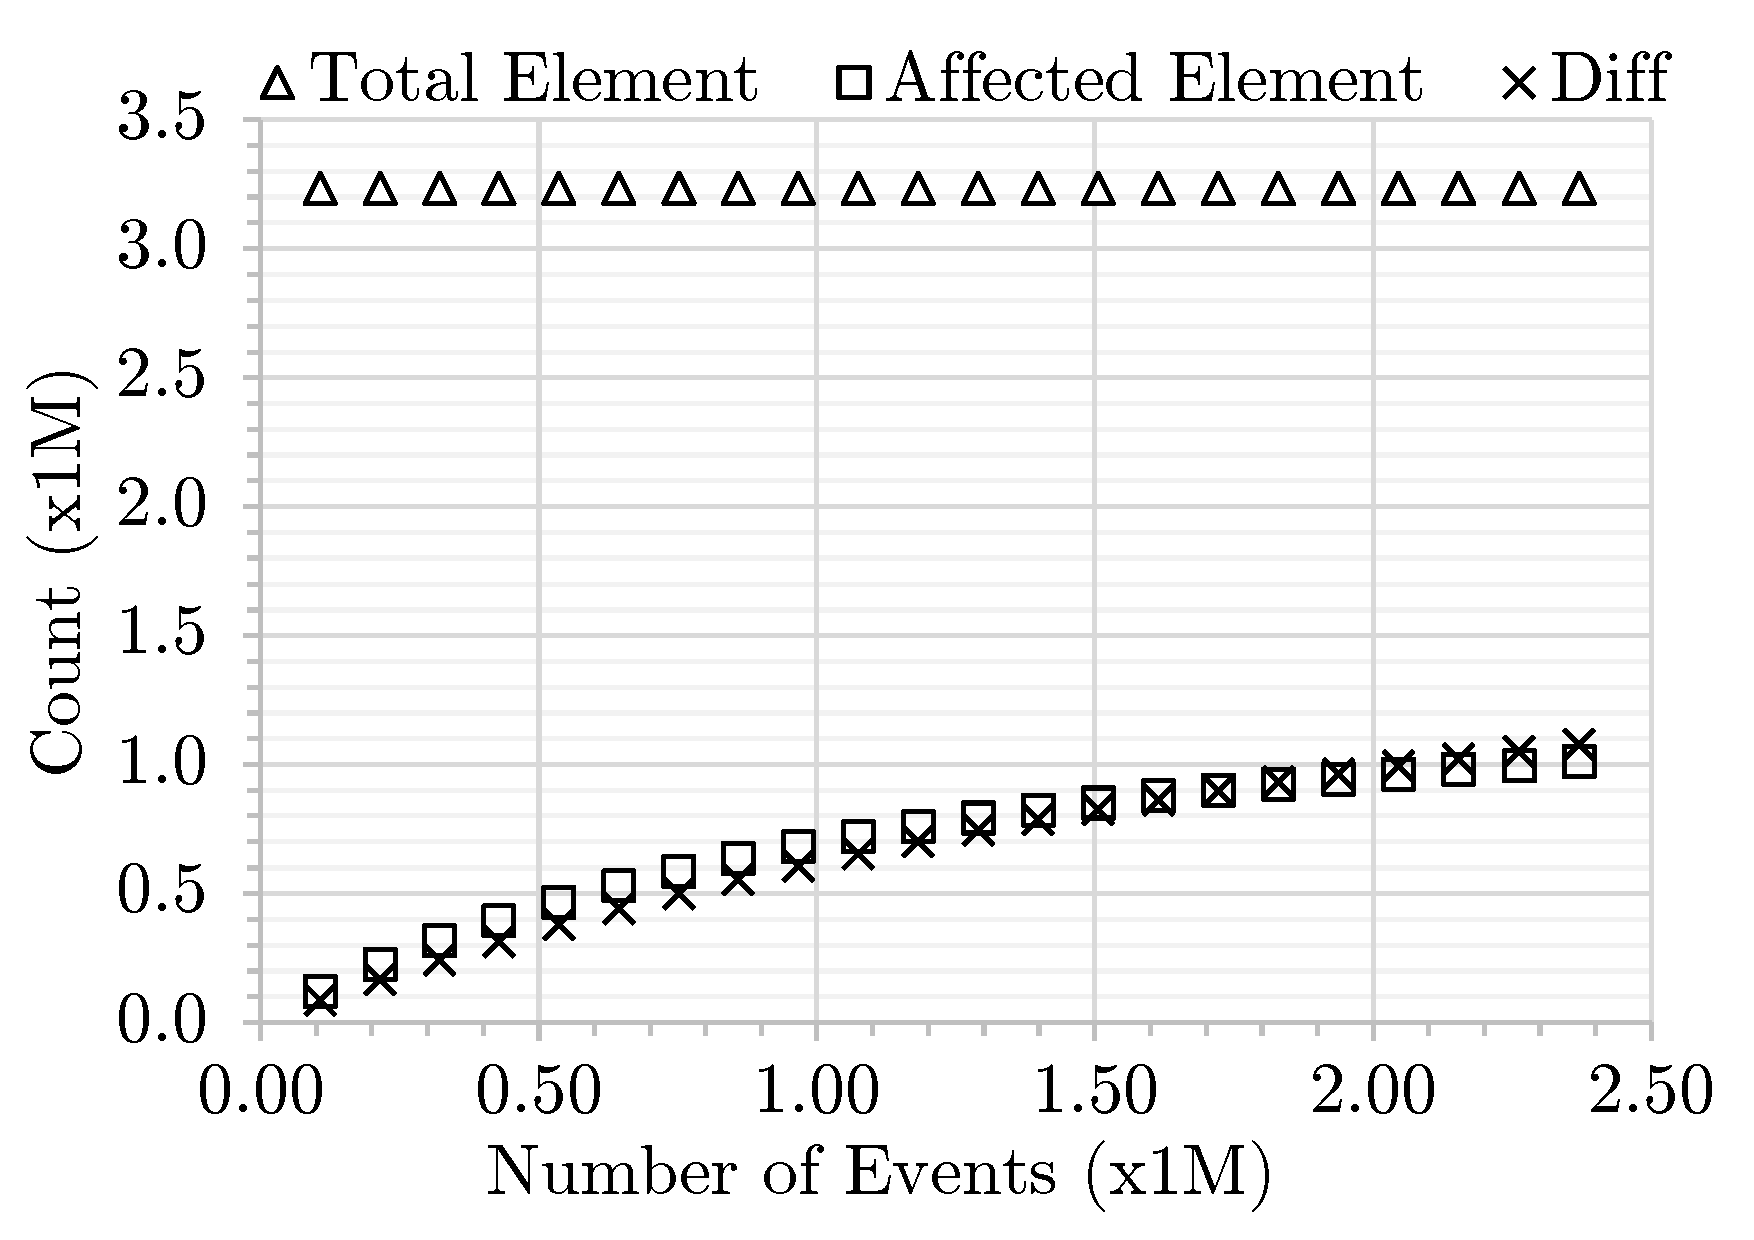
\includegraphics[width=\linewidth]{mixed-count-events}
    \caption{total elements, affected elements, and diffs}
    \label{fig:modification_course}
    \begin{subfigure}[t]{\linewidth}
        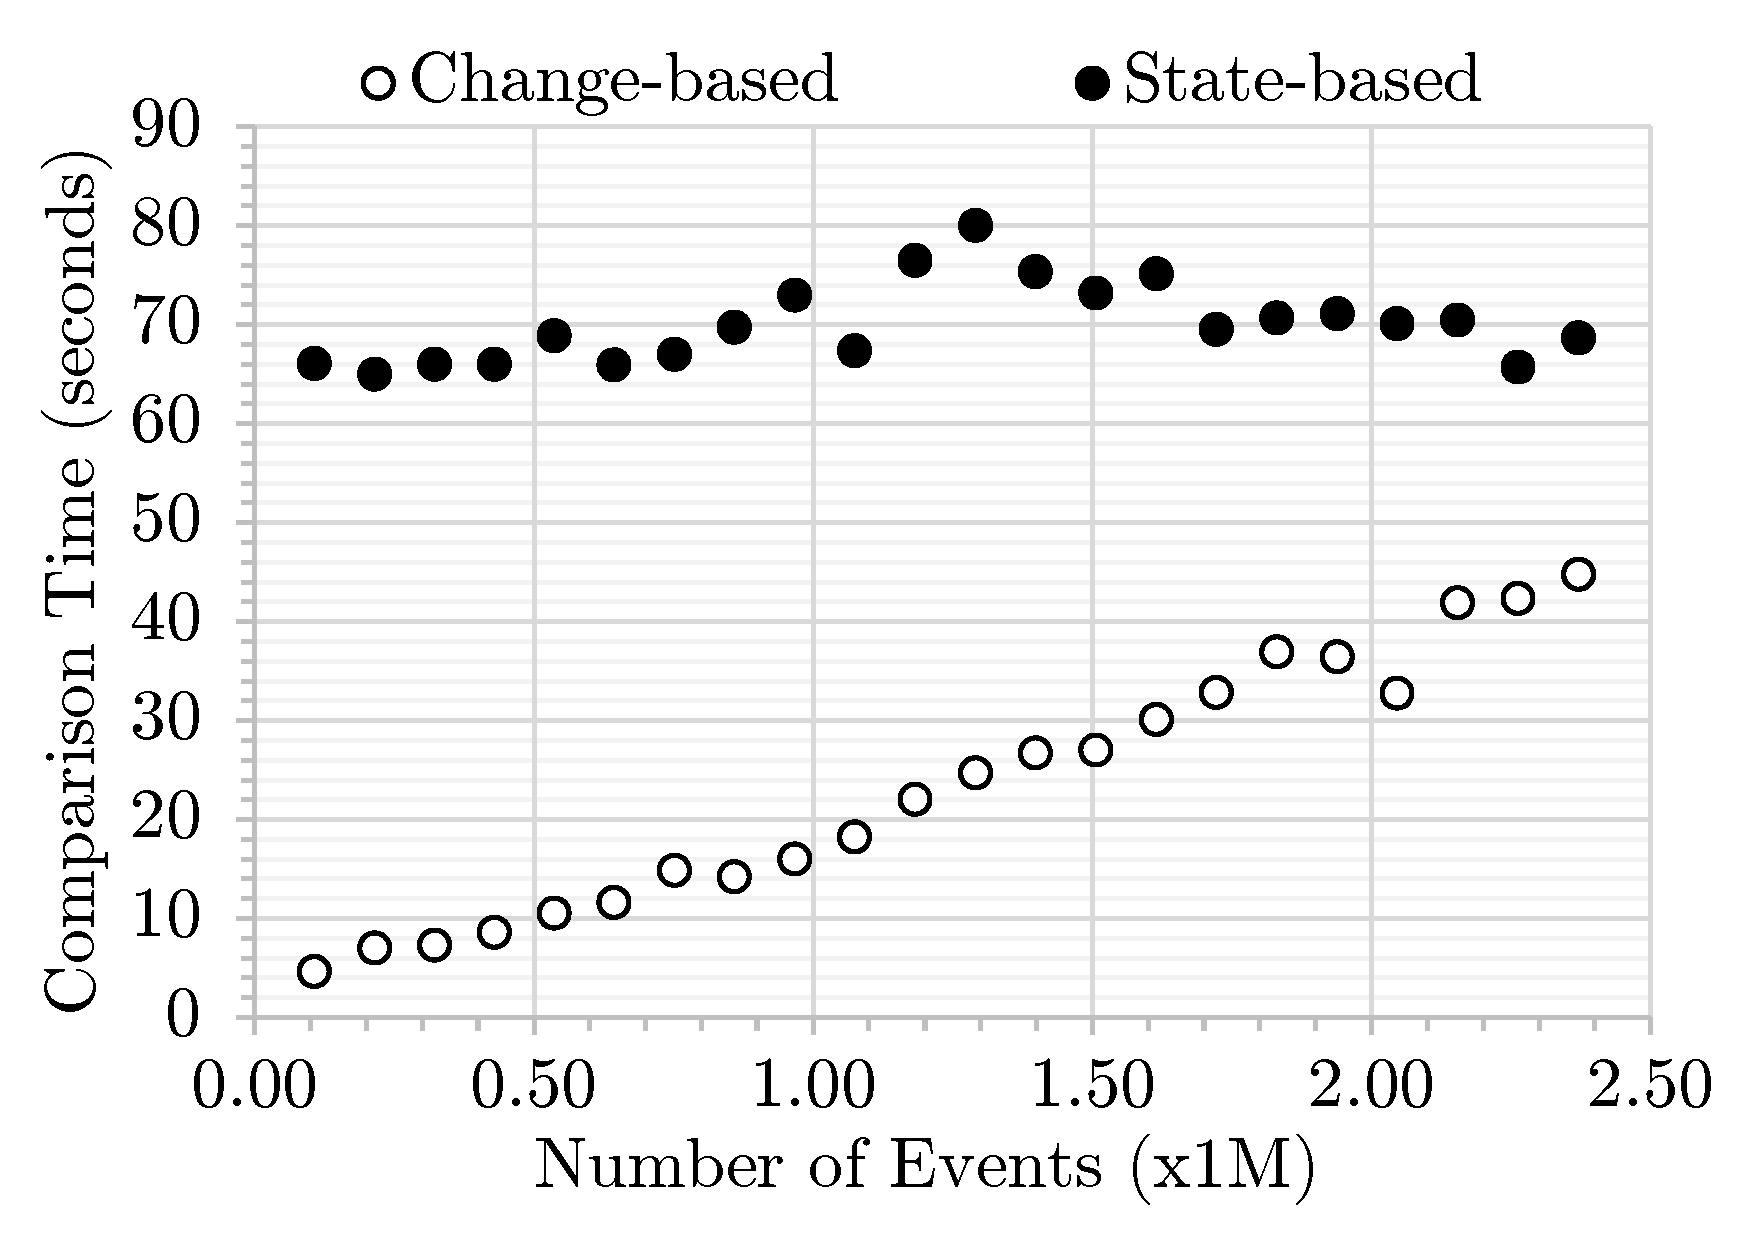
\includegraphics[width=\linewidth]{mixed-time-events}
        \caption{execution time}
        \label{fig:time_diffs}
    \end{subfigure}
    \begin{subfigure}[t]{\linewidth}
        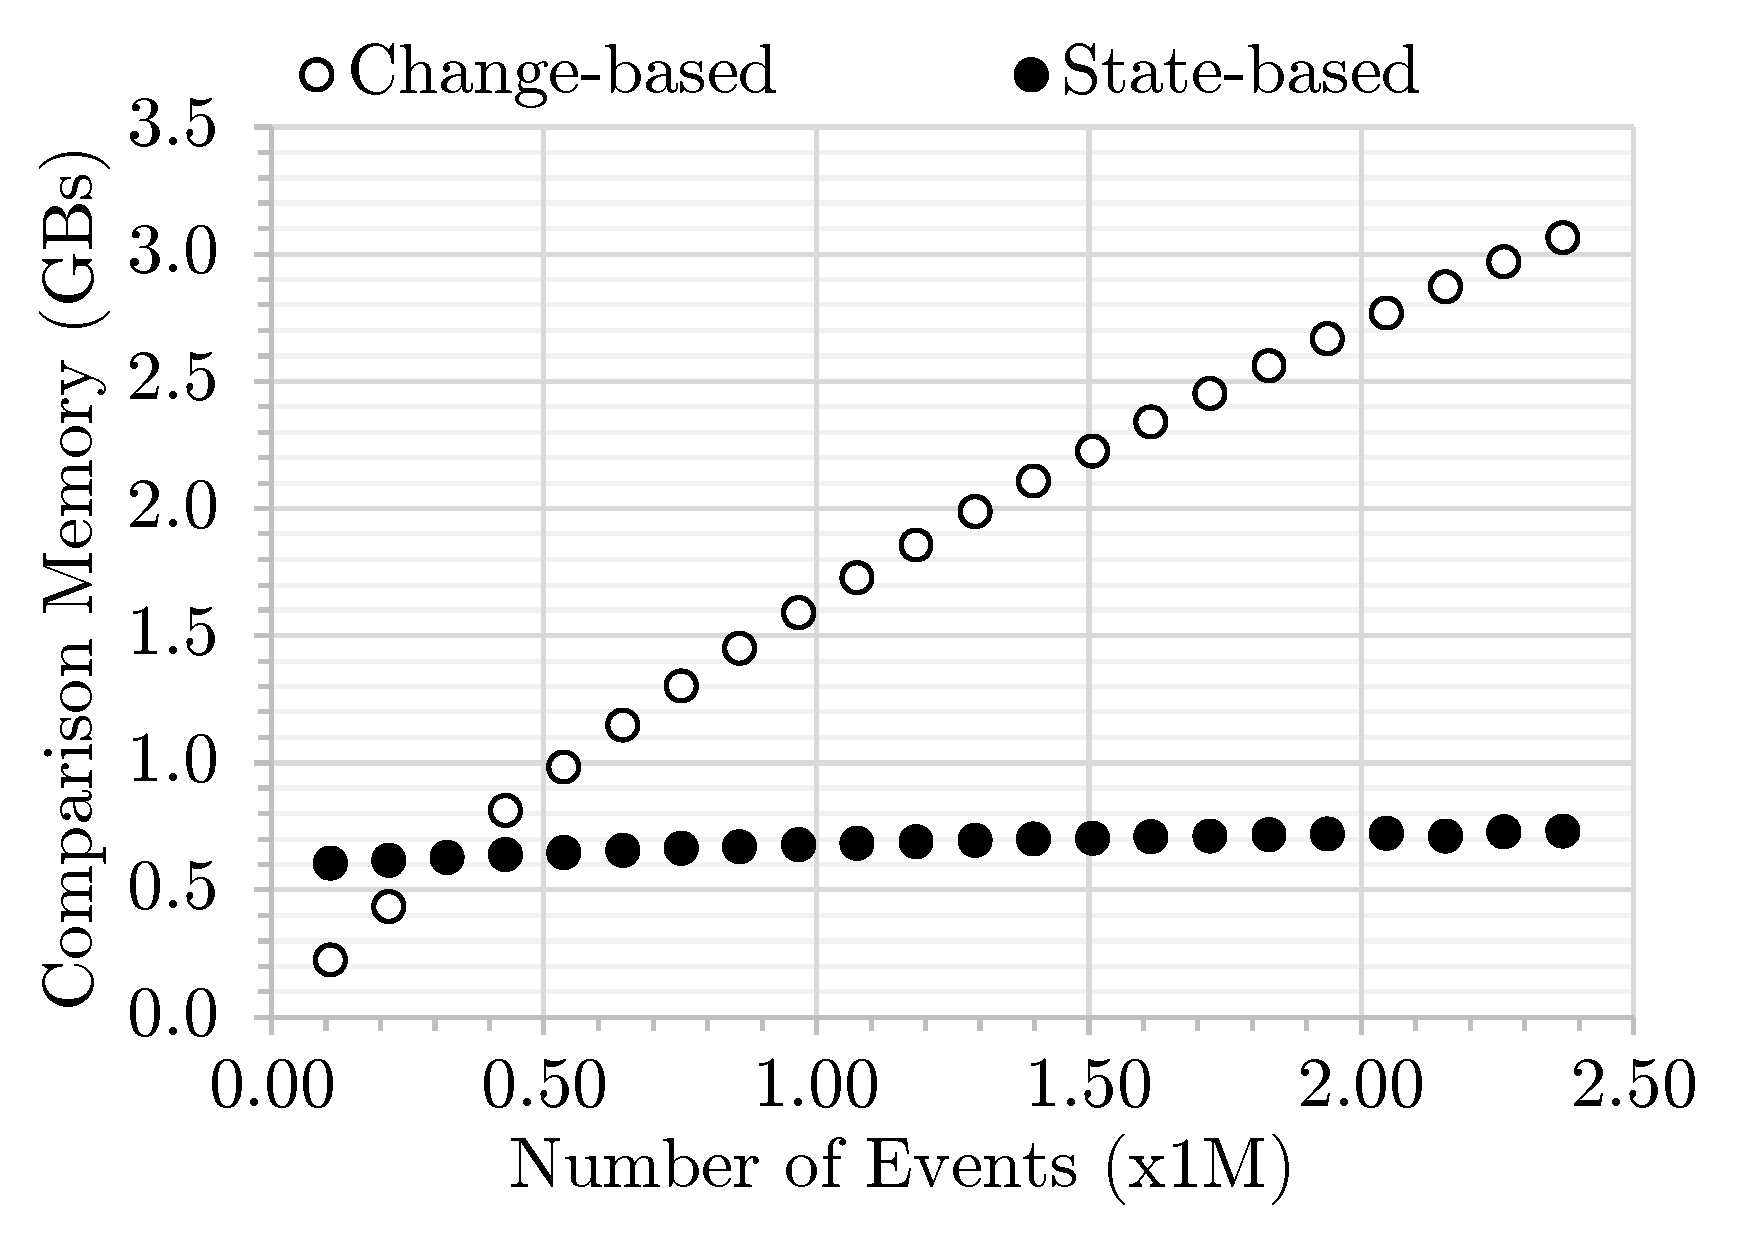
\includegraphics[width=\linewidth]{mixed-memory-events}
        \caption{memory footprint}
        \label{fig:memory_diffs}
    \end{subfigure}
    \caption{Change-based vs. state-based model comparison as differences increase.}
    \label{fig:change_vs_state}
\end{wrapfigure}

\vspace{-5pt}
\subsection{Result and Discussion}
\label{sec:discussion}
In this section, we report our evaluation on comparison time and memory footprint of the mixed and homogeneous operation measurement. 

\vspace{-5pt}
\subsubsection{Mixed Operations}
\label{sec:mixed-operation}

In the mixed operation measurement, we modify two identical models differently by applying random operations. As the number of change events generated by the modification grows, the numbers of affected elements and differences also increase in logarithmic manner. The patterns can seen in Fig. \ref{fig:modification_course}. The growth are logarithmic since the probability that the random operations modify the same elements also increases. Thus, some change events might not contribute to the addition of new affected elements and differences. In other words, more events are required to increase the number of affected elements or differences. In Fig. \ref{fig:modification_course}, the total elements is constant due to the equal probabilities of addition and deletion as has been set in Section \ref{sec:evaluation}. The figure gives us an insight about the characteristics of the modification caused by the random operations in the mixed operation measurement; it supports explaining the implication of the changes on execution time and memory footprints of model comparison.

After applying some random changes on both models, the modification produces 100,000 change events at the first measurement point. Using this amount of events, our change-based comparison only takes 5 seconds to identify around 90,000 differences, in contrast to the state-based comparison that takes 66 seconds (see the first measurement points in Figures \ref{fig:modification_course} and \ref{fig:time_diffs}). If the modification continues, more changes events are generated. This growing number of change events has to be loaded into memory and thus slows down the change-based comparison. Nevertheless, the change-based comparison is still faster than the state-based comparison even though the number of change events reaches 2.37 millions -- more than 1 million differences at that point; the change-based comparison outperforms the state-based comparison in execution time (Figure \ref{fig:time_diffs}). Fig. \ref{fig:time_changediff_detail} breaks down the comparison time in detail. It exhibits that the event loading time is the dominant contributor to the slowdown compared to the element tree's construction time and diffing time. 

\begin{figure}[ht]
    \centering
    \begin{subfigure}[t]{0.495\linewidth}
        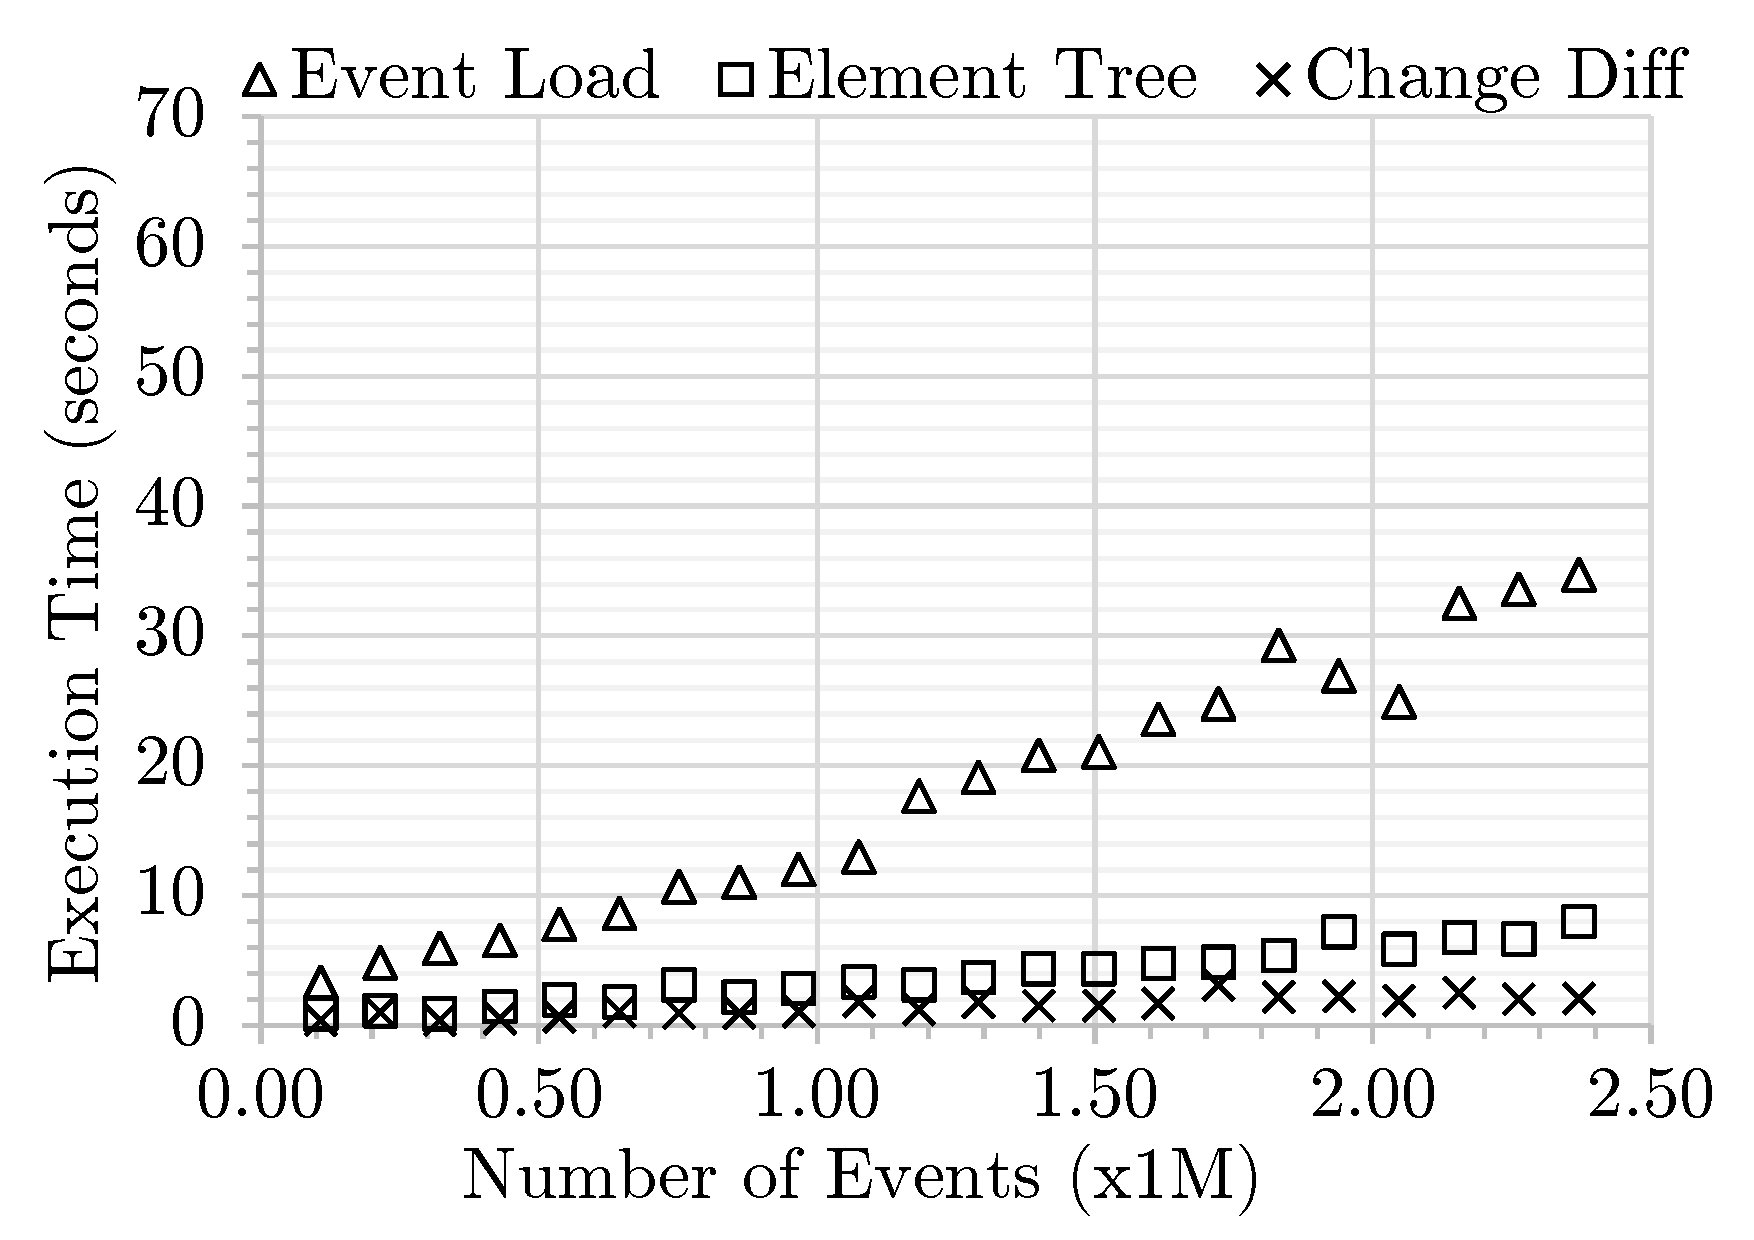
\includegraphics[width=\linewidth]{mixed-time-events-detail}
        \caption{change-based comparison time}
        \label{fig:time_changediff_detail}
    \end{subfigure}
    \hfill
    \begin{subfigure}[t]{0.495\linewidth}
        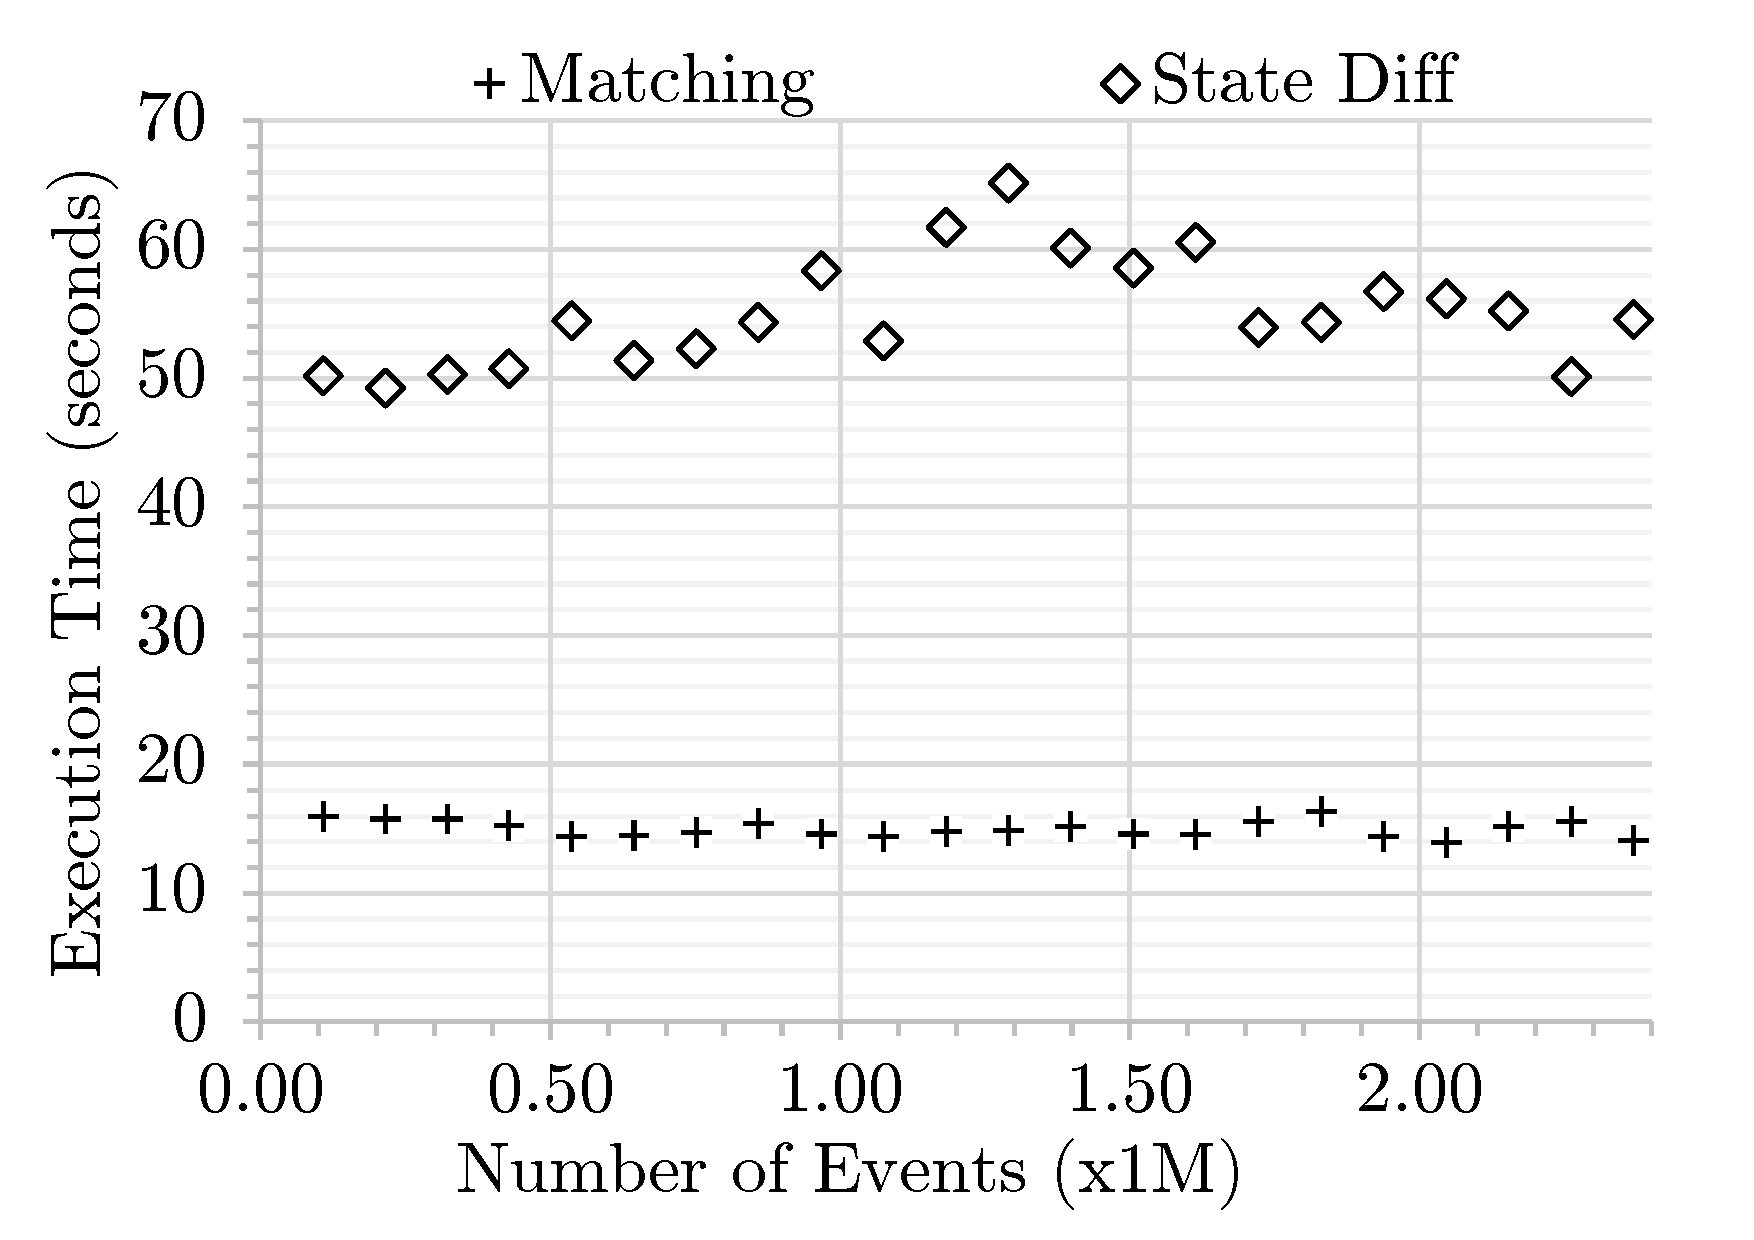
\includegraphics[width=\linewidth]{state-time-events-detail}
        \caption{state-based comparison time}
        \label{fig:time_statediff_detail}
    \end{subfigure}
    \begin{subfigure}[t]{0.495\linewidth}
        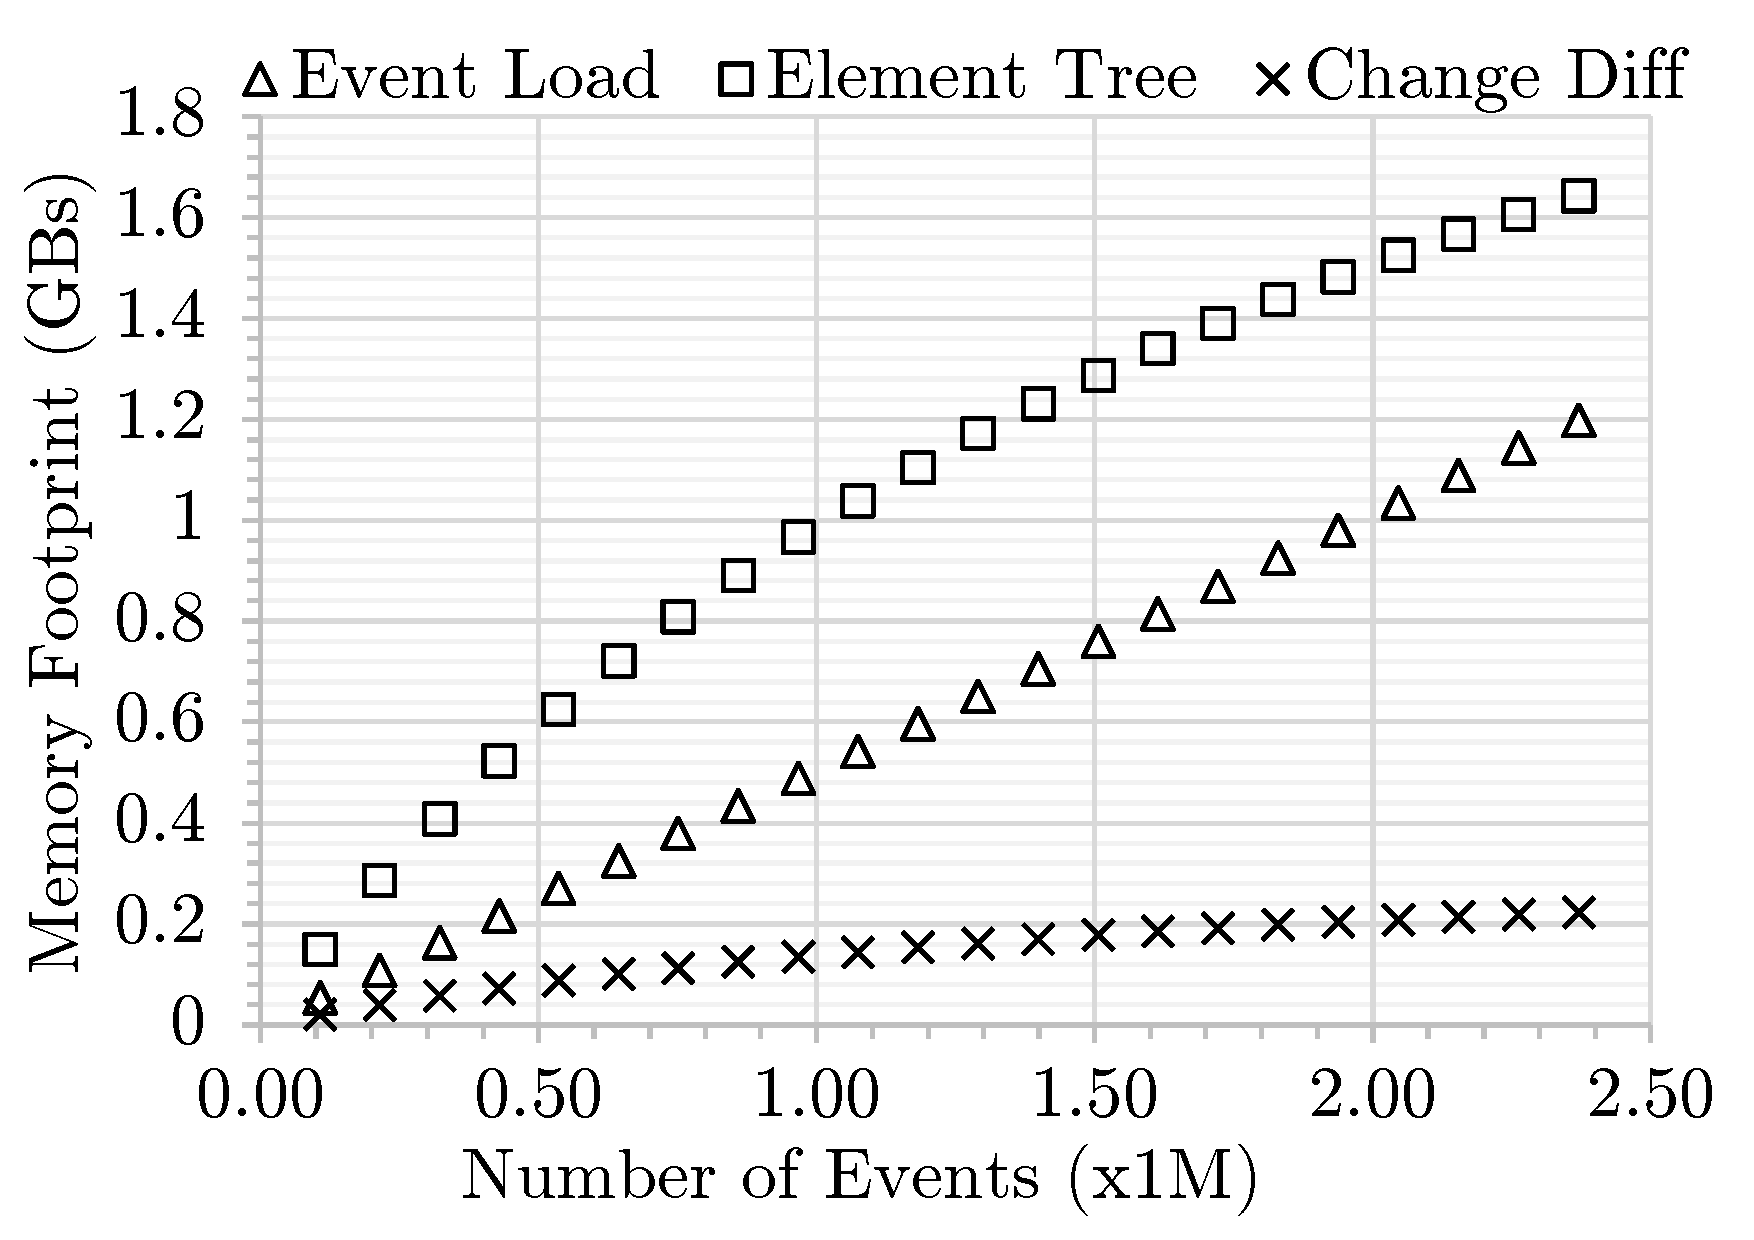
\includegraphics[width=\linewidth]{mixed-memory-events-detail}
        \caption{change-based memory footprint}
        \label{fig:memory_changediff_detail}
    \end{subfigure}
    \hfill
    \begin{subfigure}[t]{0.495\linewidth}
        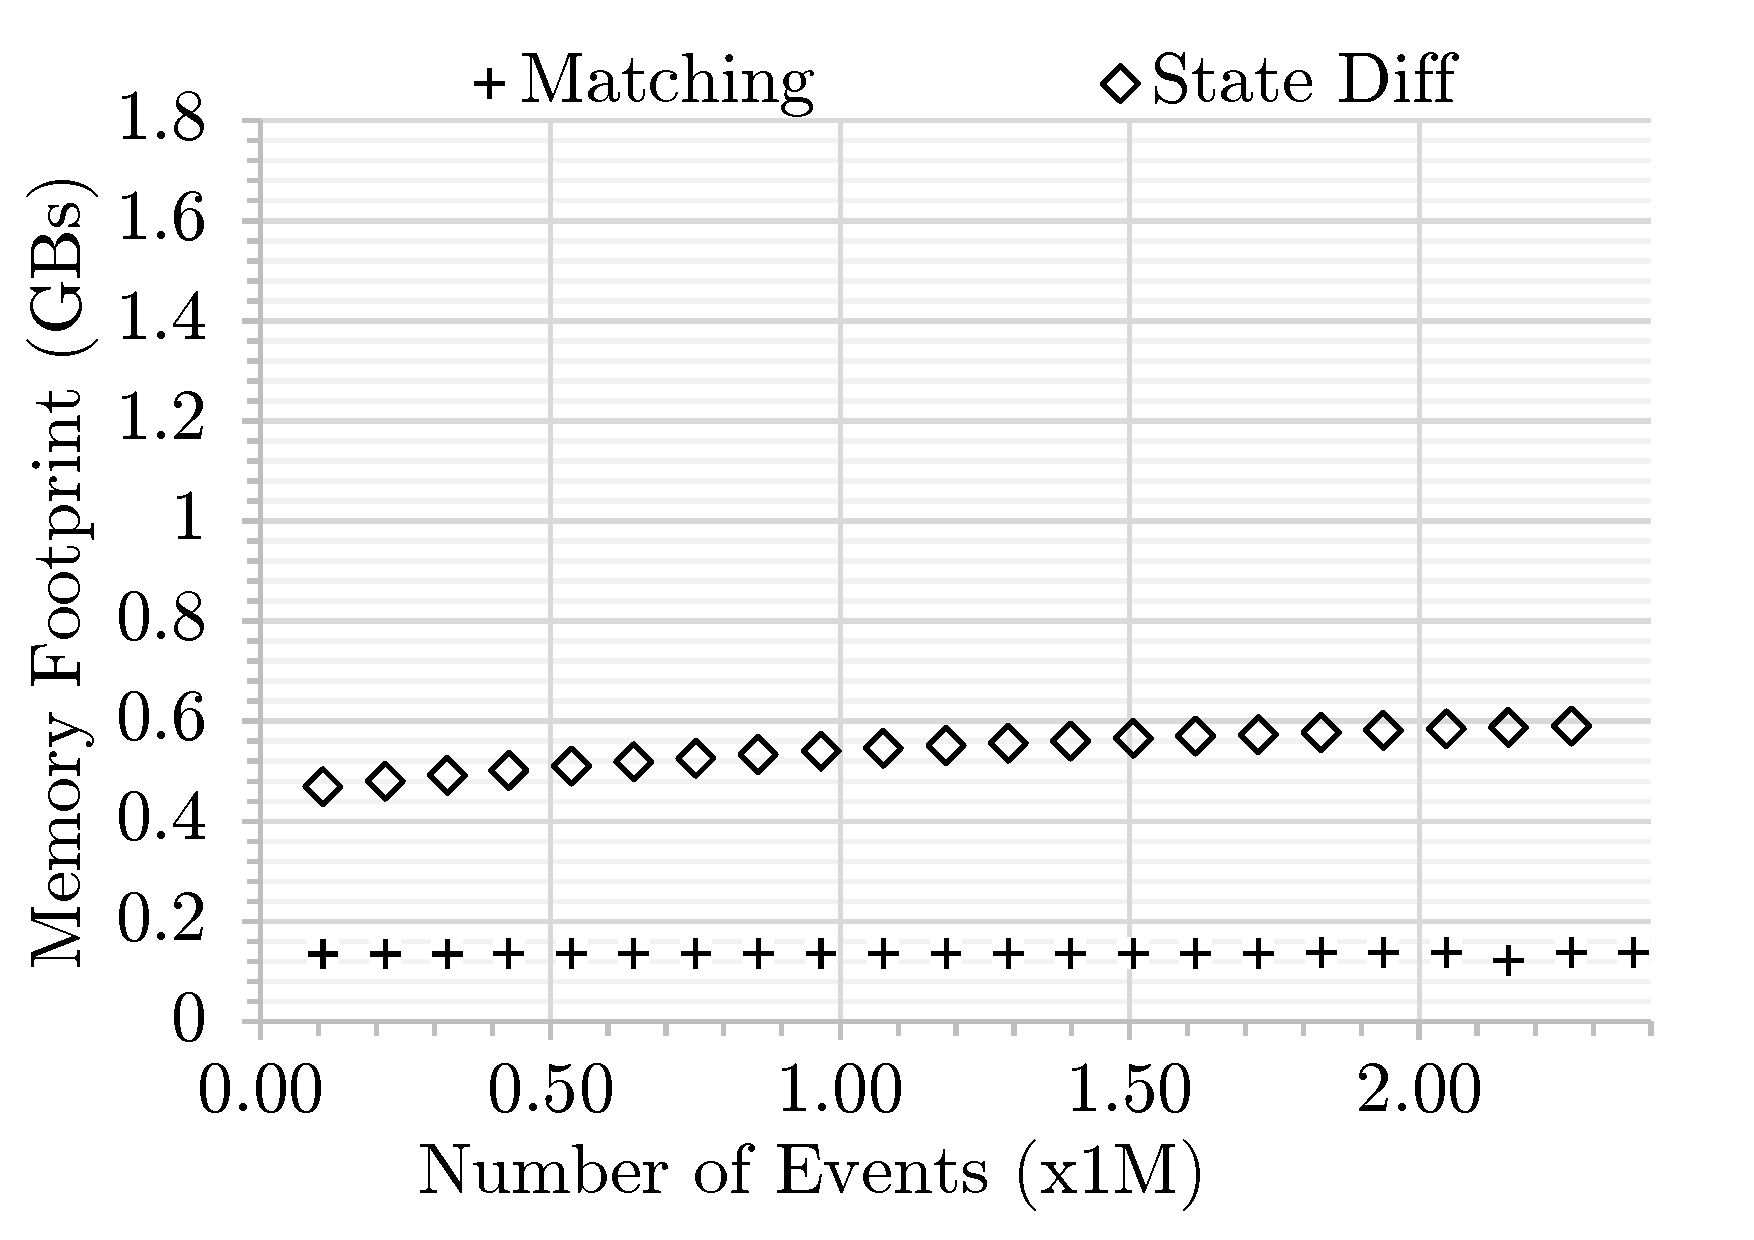
\includegraphics[width=\linewidth]{state-memory-events-detail}
        \caption{state-based memory footprint}
        \label{fig:memory_statediff_detail}
    \end{subfigure}
    \caption{Breakdown view of comparison time and memory footprint in Figure \ref{fig:change_vs_state}.}
    \label{fig:time_memory_detail}
\end{figure}

For the state-based comparison in Fig. \ref{fig:time_statediff_detail}, the comparison time only experiences a slight increase as the number of identified differences also inclines. This slight increase is contributed mainly by the diffing time, while the matching time tends to be constant due to the very small increase of the total elements (Figures \ref{fig:modification_course}).

Nevertheless, the change-based comparison also comes with a drawback on memory footprint since it consumes more space than the state-based comparison does (see Figure \ref{fig:memory_diffs}). The change-based comparison only consumes less memory than its state-based counterpart when the number of events is less than 0.3 millions (around less than 0.25 million identified differences at that moment). Fig. \ref{fig:memory_changediff_detail} breaks down the memory footprint of the change-based comparison into three factors: the loaded change events, element tree, and diffs. As modification continues, an increasing number of events is generated. These events have to be loaded into memory since they contain the required information for the construction of an element tree. The amount of space to keep these change events in memory grows linearly according to their number. 

In contrast, the memory used for the element tree grows in logarithmic pattern. As the number of events increases, the probability of the events modifies elements that already affected also increases. Thus, no additional memory allocation is required for the element tree. We can also notice that the element tree occupies most of the memory footprint since it mimics the partial states -- elements, features, and values -- of the models that are affected by the changes. Moreover, in our technical implementation, a feature can have many instances -- one instance for each element (As a comparison, in the EMF implementation, there is only one instance for a feature. The feature is used as a key so that different elements can have the same feature that maps to different values simultaneously). This contributes to the large memory footprint used by the element three. The identified change-based diffs, the third factor, are the smallest factor that contributes to the memory footprint of the change-based comparison. 

For the state-based comparison in Fig. \ref{fig:memory_statediff_detail}, the memory footprint only inclines slightly along the increase of differences. A large part of the memory footprint is used to represent the identified differences, while the memory used for matches tends to be constant as the changes of the total elements are very small -- less new elements means less memory needs to be allocated for new matches (Figures \ref{fig:modification_course}). 

\subsubsection{Homogeneous Operations}
\label{sec:homogeneous-operation}

\begin{figure}[ht]
    \centering
    \begin{subfigure}[t]{0.495\linewidth}
        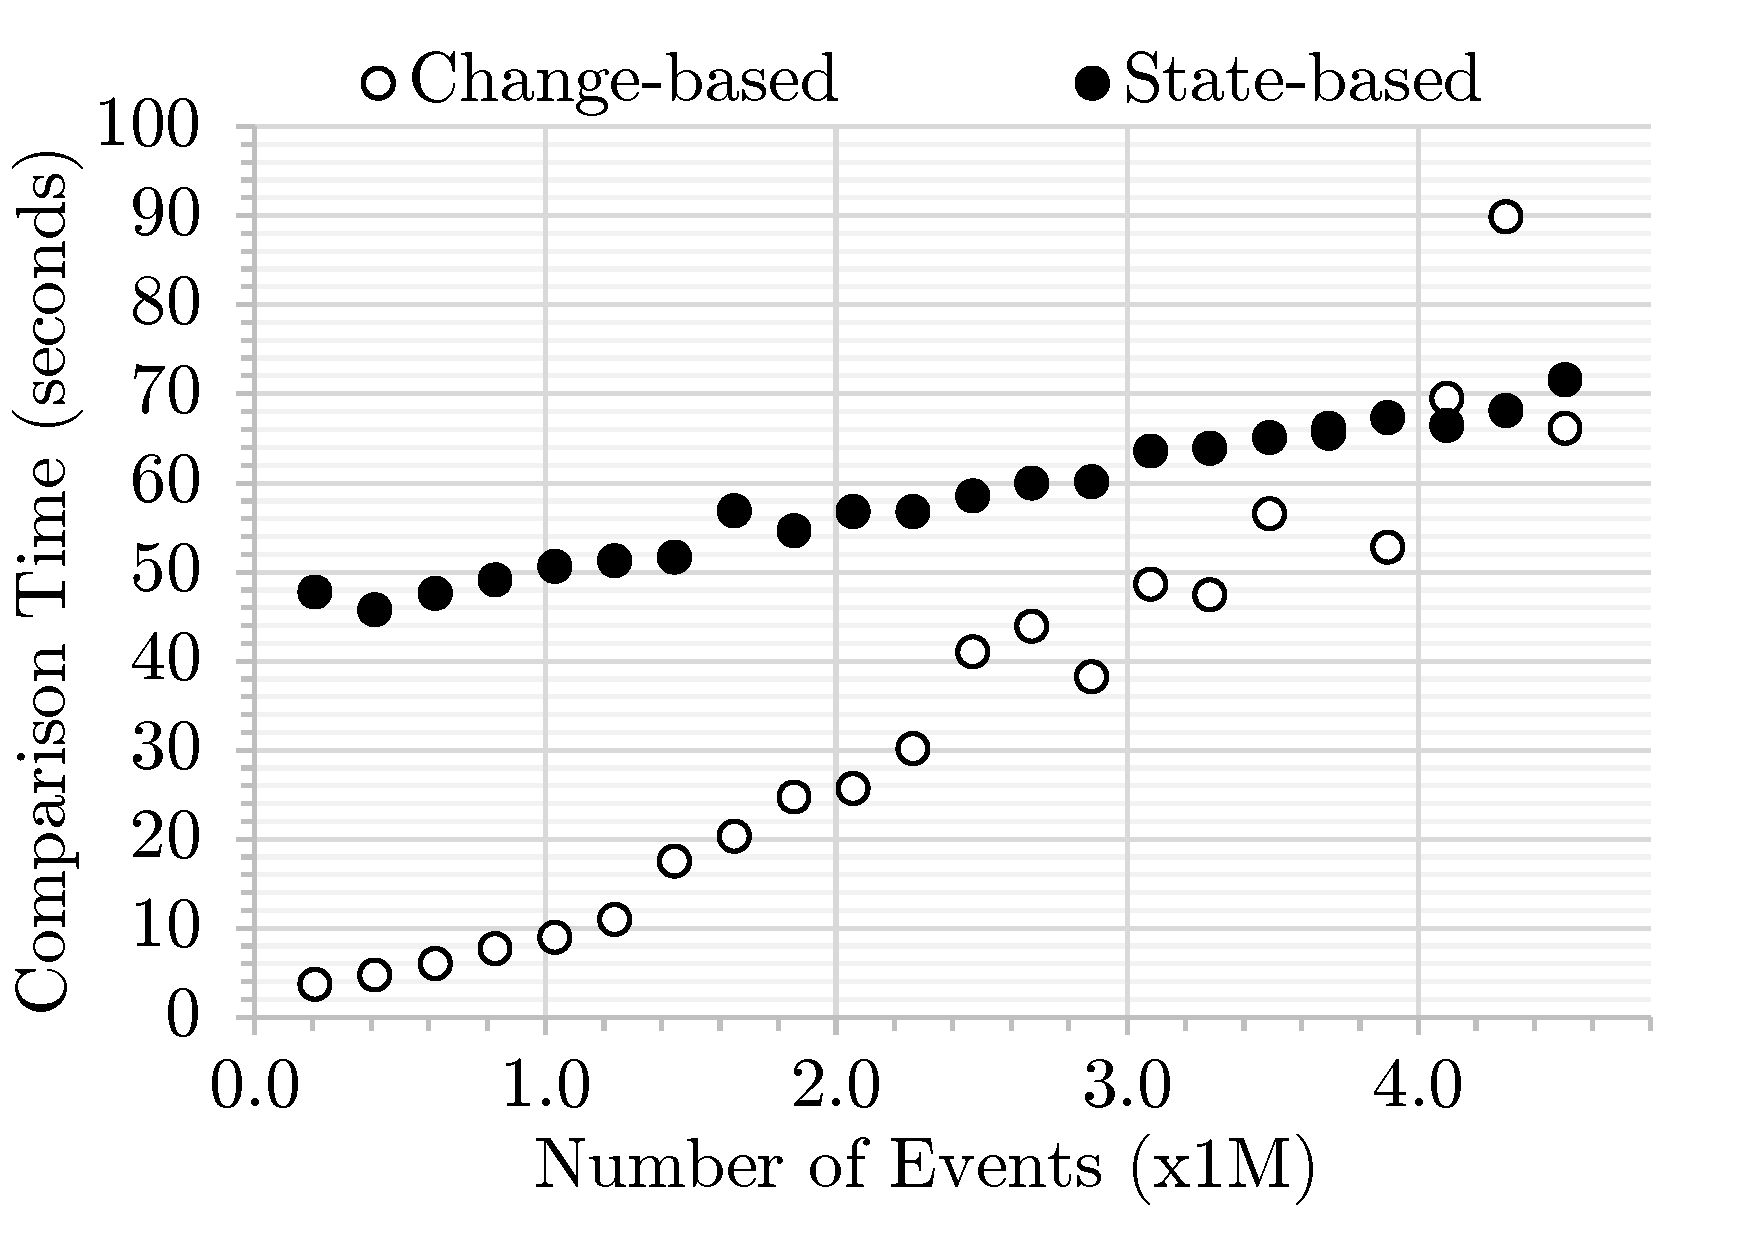
\includegraphics[width=\linewidth]{add-time-events}
        \caption{add-only}
        \label{fig:add-time-events}
    \end{subfigure}
    \hfill
    \begin{subfigure}[t]{0.495\linewidth}
        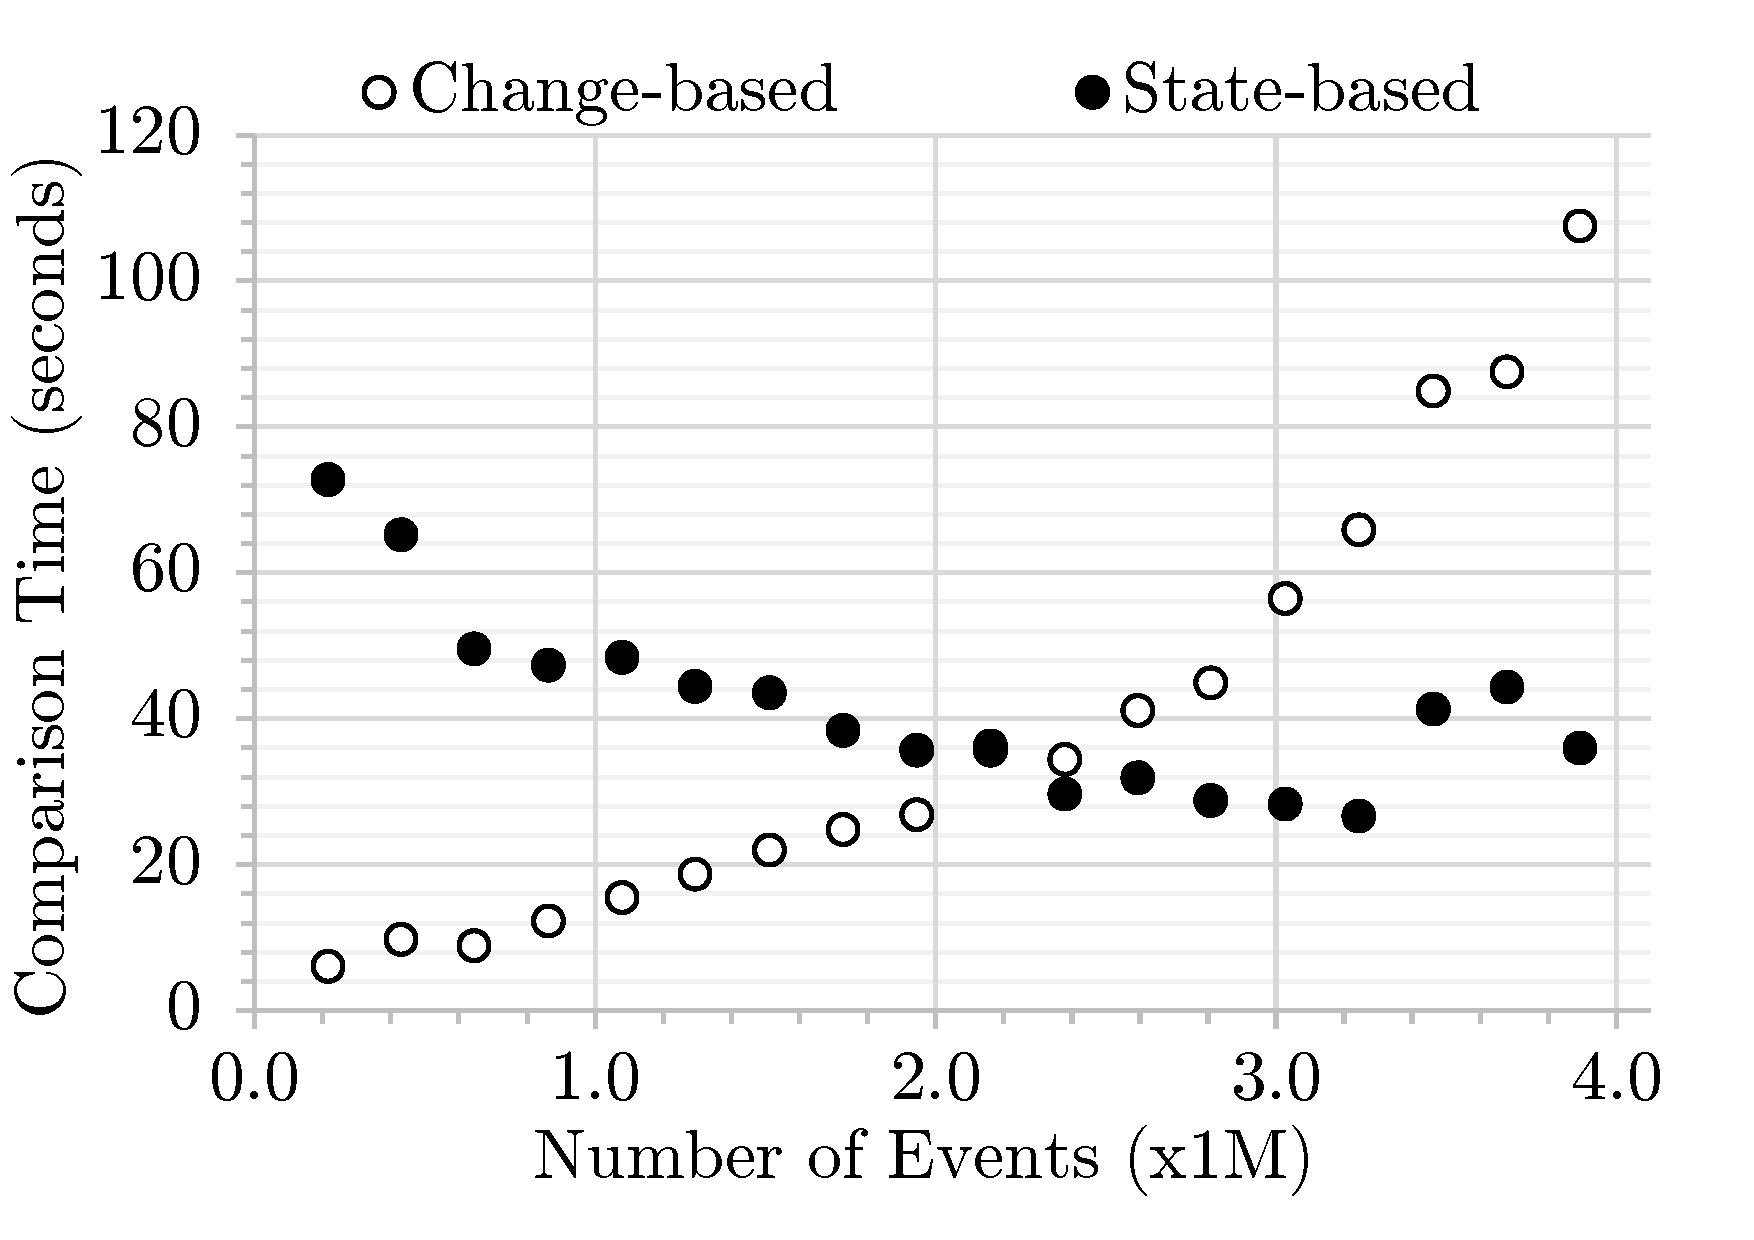
\includegraphics[width=\linewidth]{delete-time-events}
        \caption{delete-only}
        \label{fig:delete-time-events}
    \end{subfigure}
    \begin{subfigure}[t]{0.495\linewidth}
        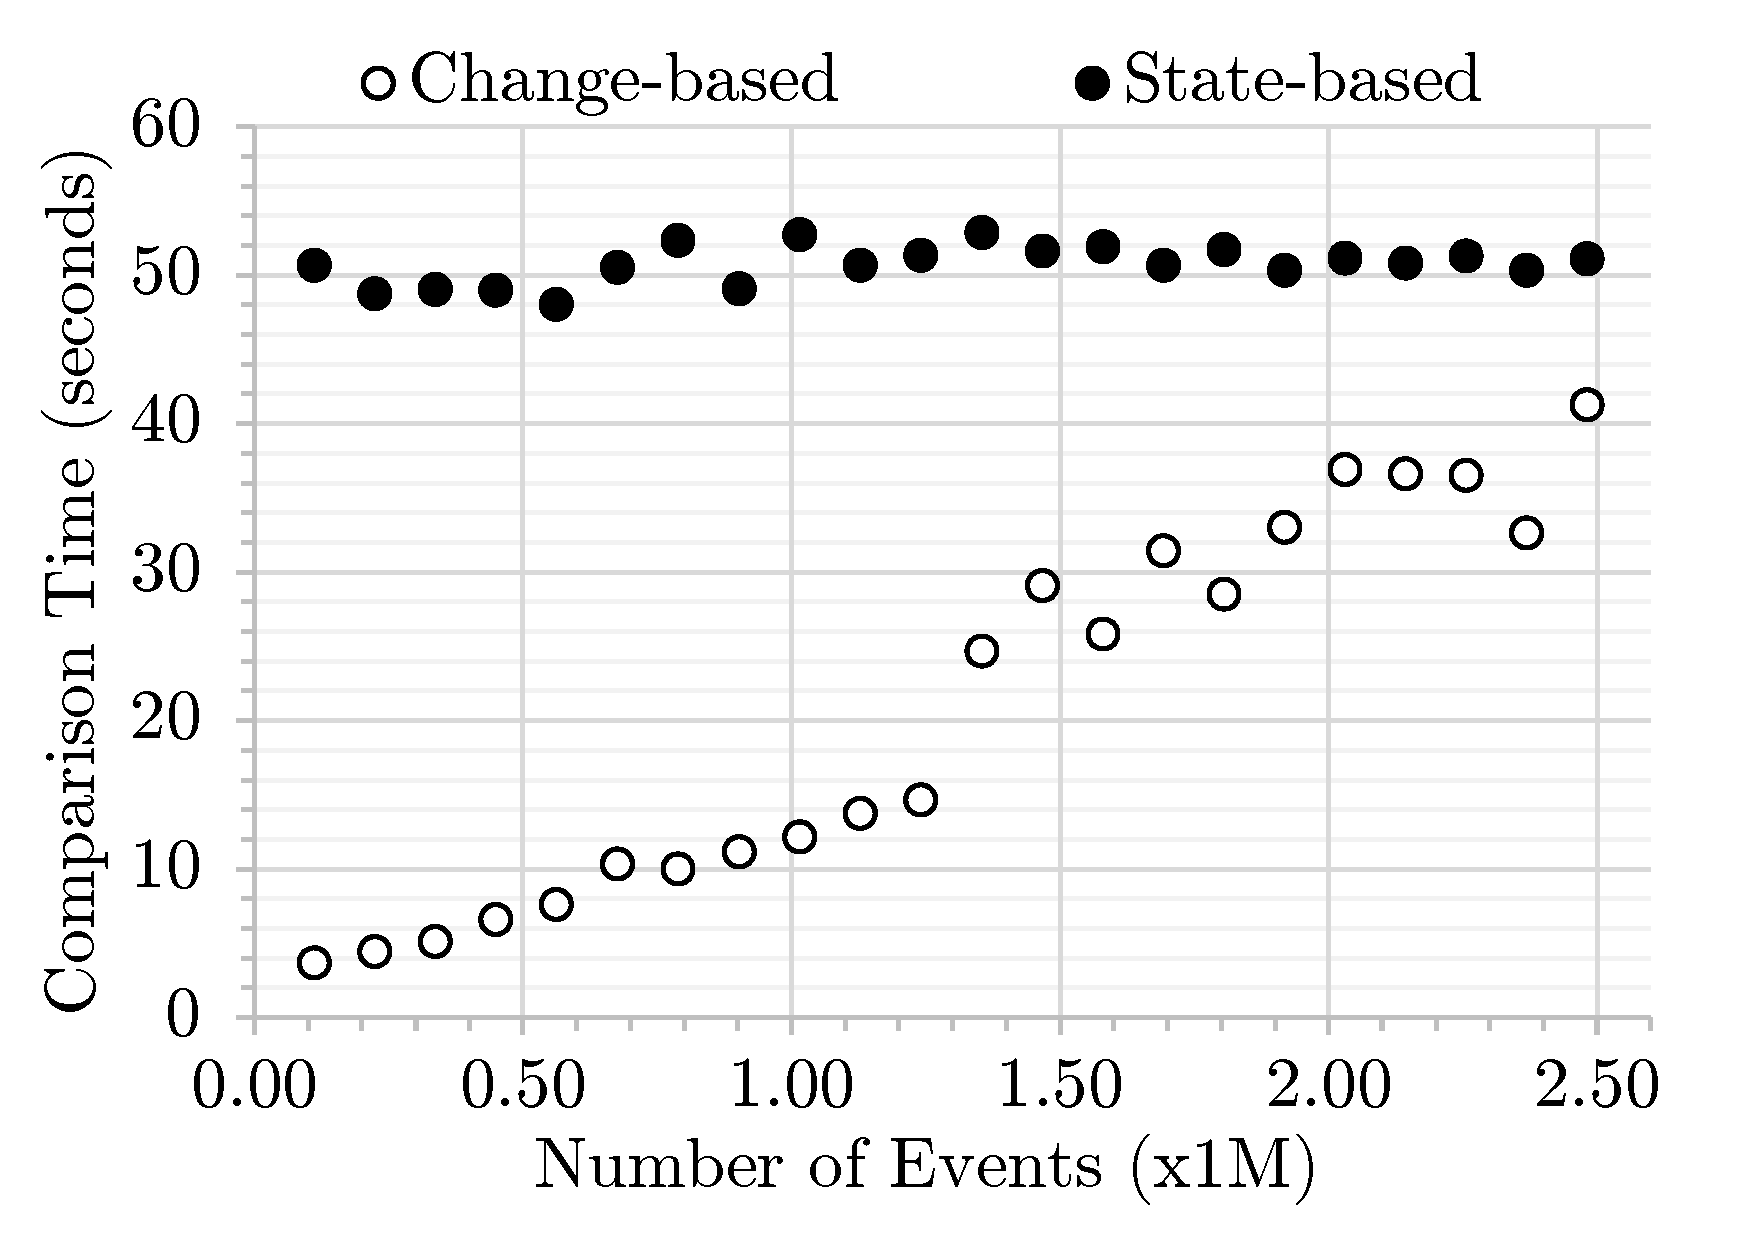
\includegraphics[width=\linewidth]{move-time-events}
        \caption{move-only}
        \label{fig:move-time-events}
    \end{subfigure}
    \hfill
    \begin{subfigure}[t]{0.495\linewidth}
        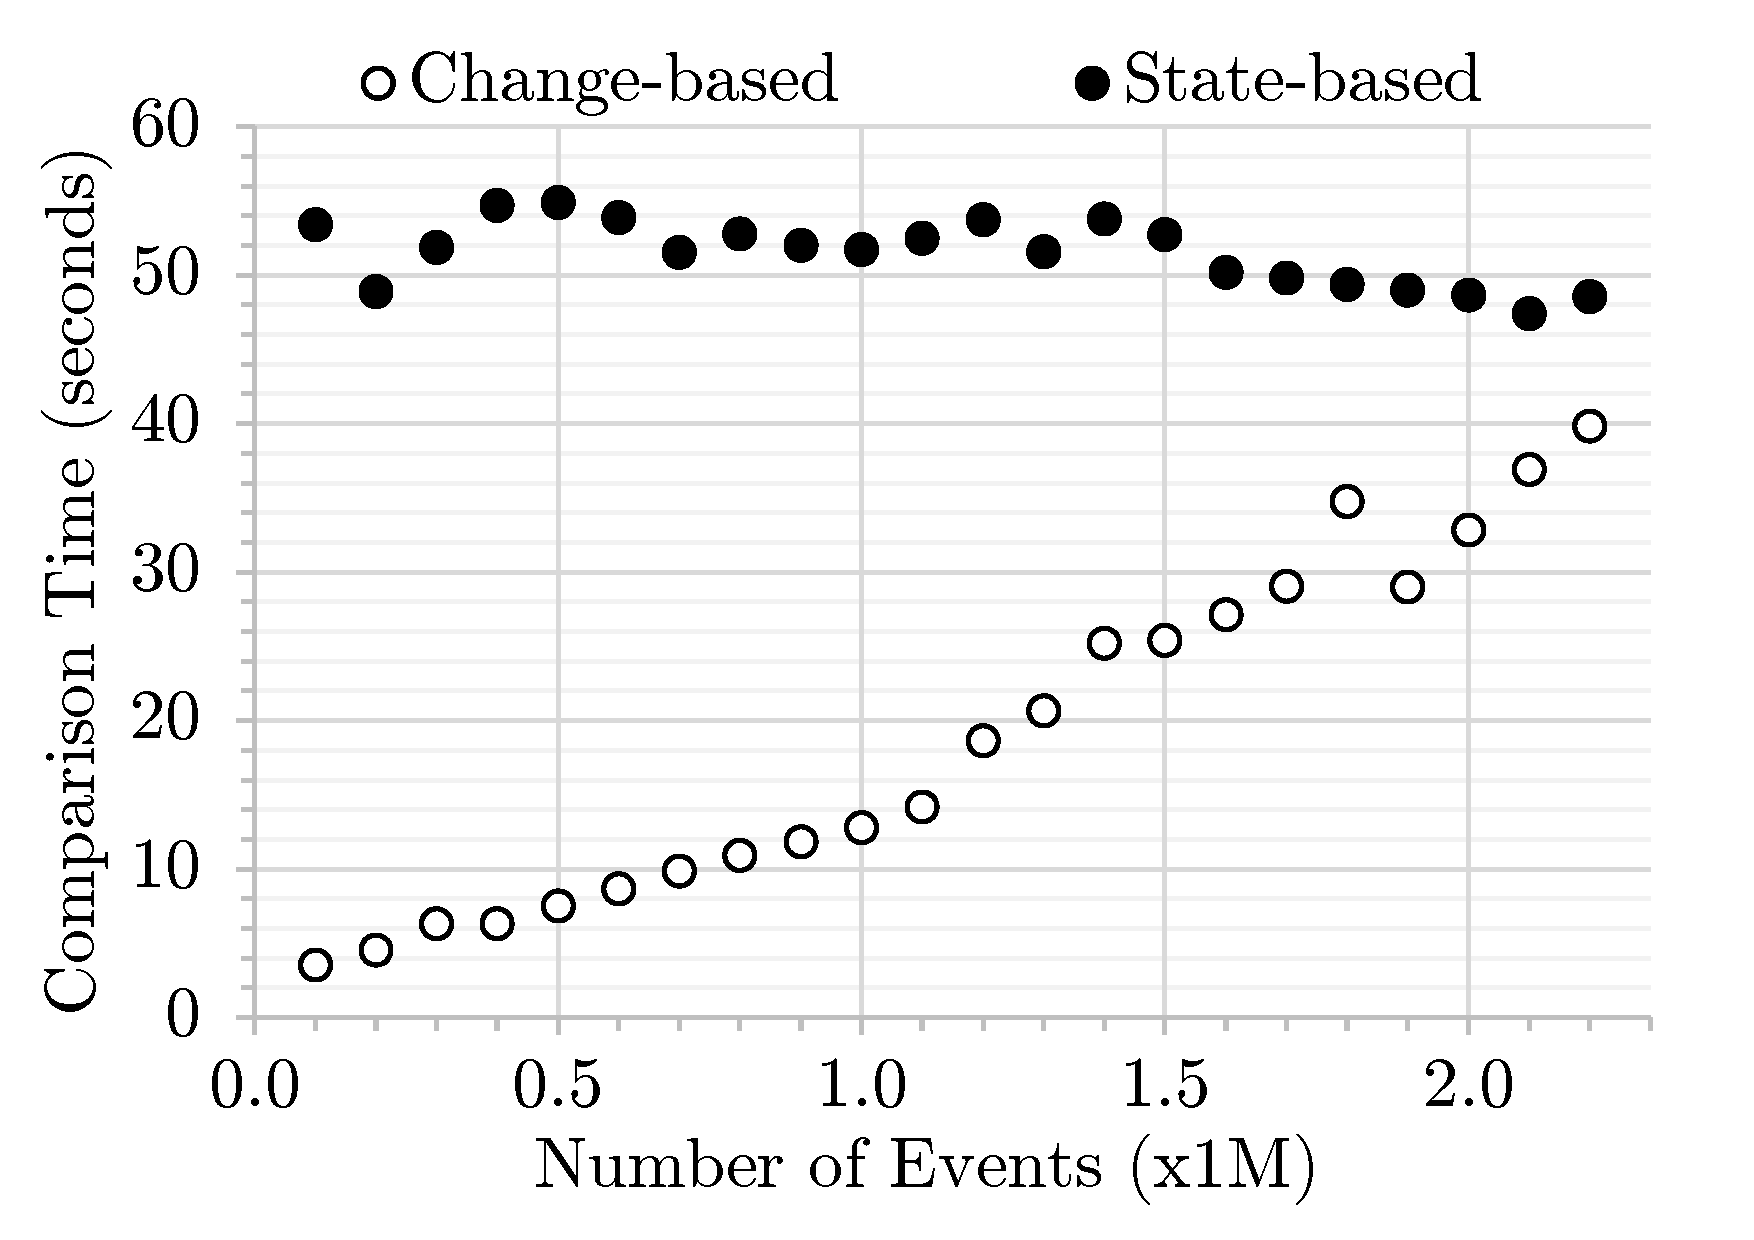
\includegraphics[width=\linewidth]{change-time-events}
        \caption{change-only}
        \label{fig:change-time-events}
    \end{subfigure}
    \caption{Comparison time for homogeneous operations.}
    \label{fig:operation_time_events}
\end{figure}

\begin{figure}[ht]
    \centering
    \begin{subfigure}[t]{0.495\linewidth}
        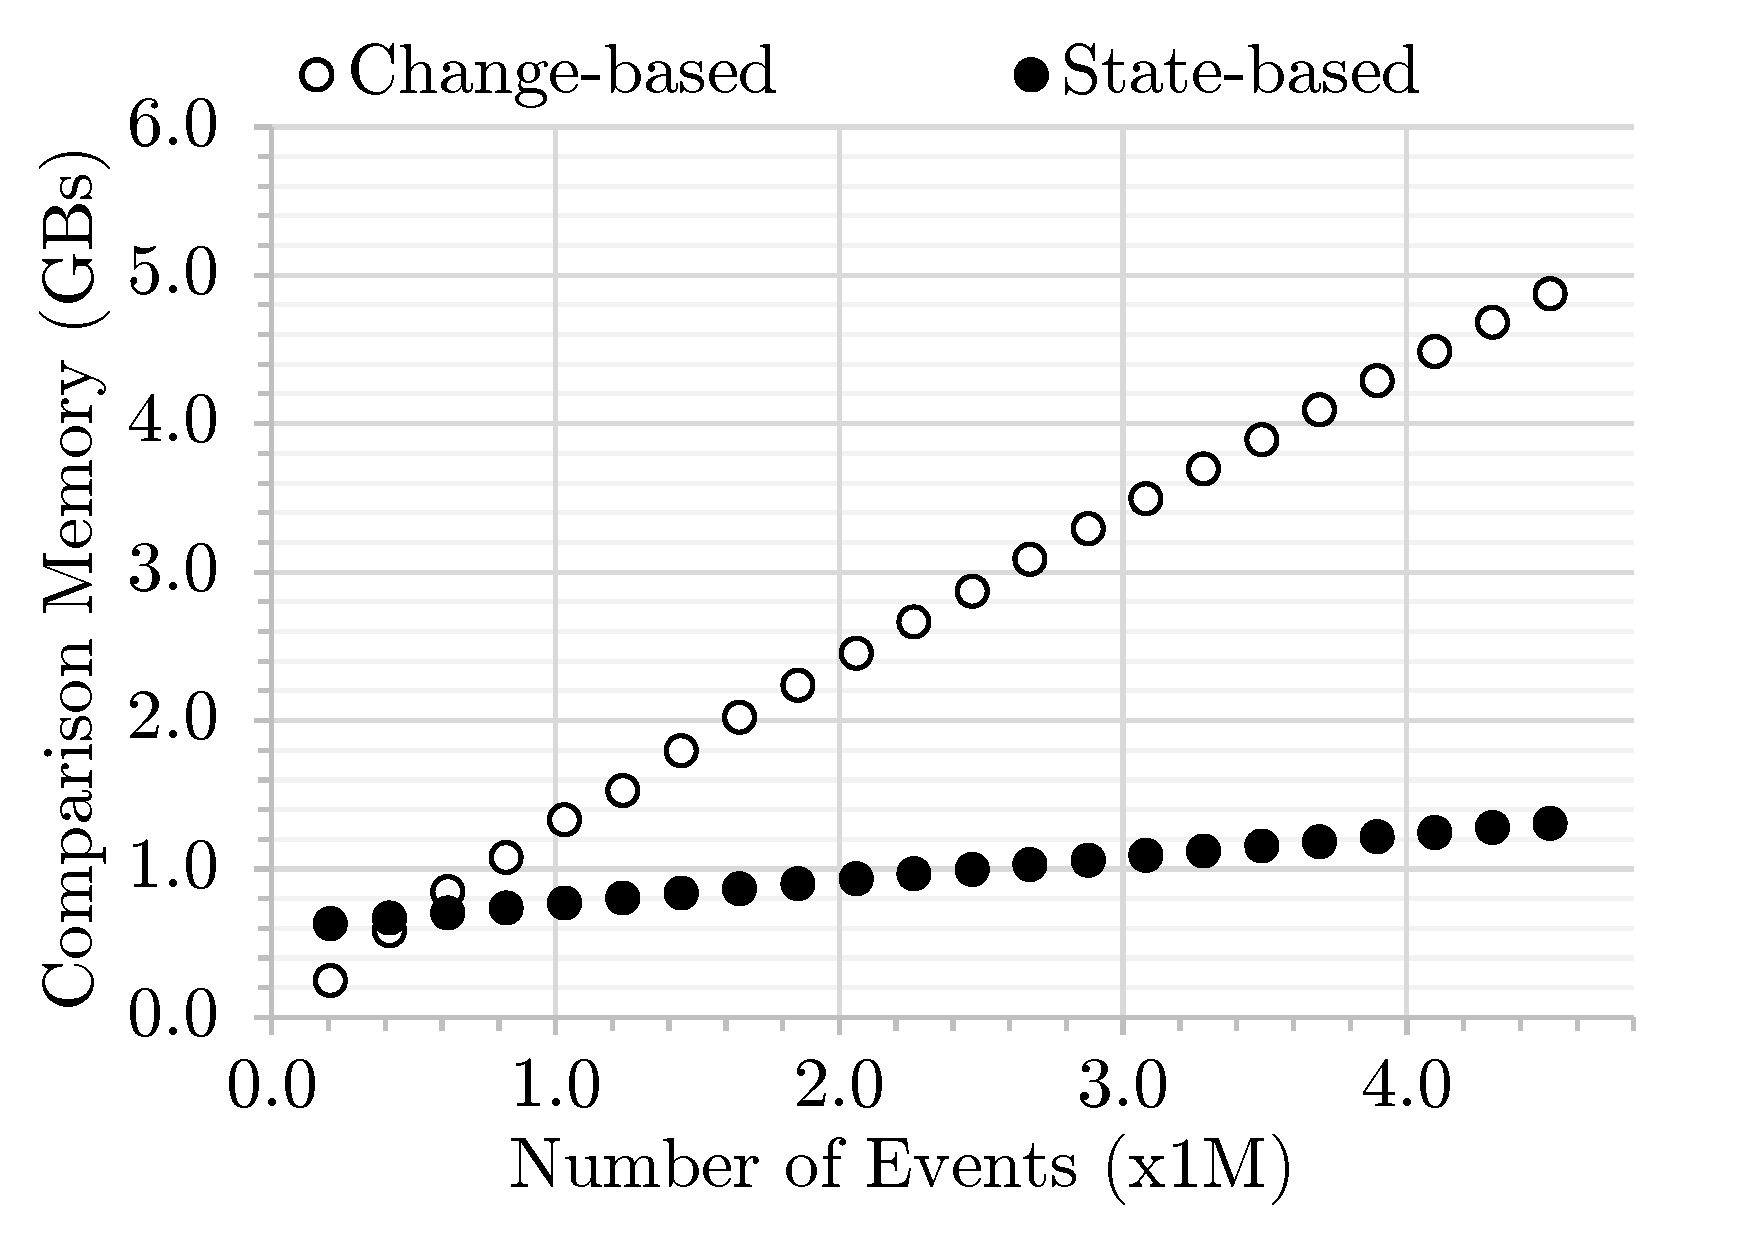
\includegraphics[width=\linewidth]{add-memory-events}
        \caption{add-only}
        \label{fig:add-memory-events}
    \end{subfigure}
    \hfill
    \begin{subfigure}[t]{0.495\linewidth}
        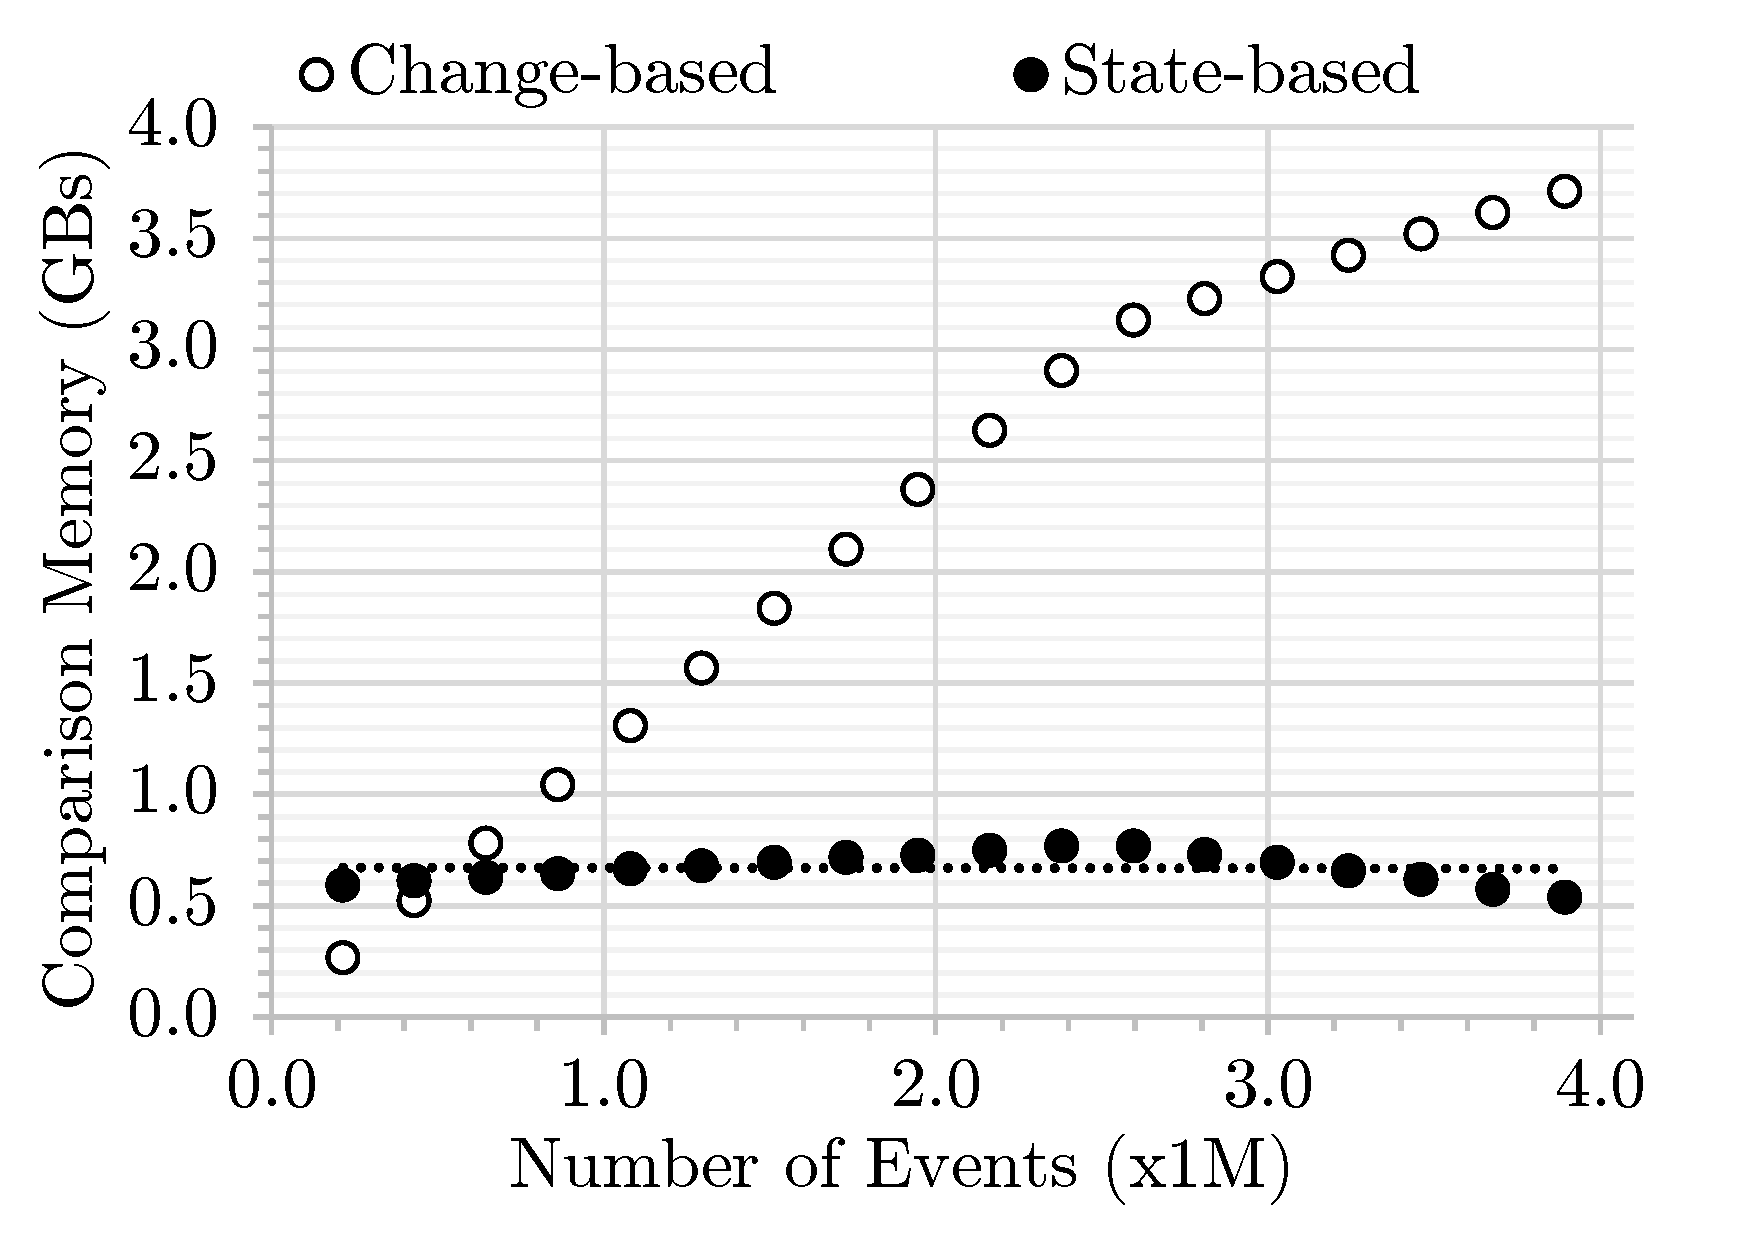
\includegraphics[width=\linewidth]{delete-memory-events}
        \caption{delete-only}
        \label{fig:delete-memory-events}
    \end{subfigure}
    \begin{subfigure}[t]{0.495\linewidth}
        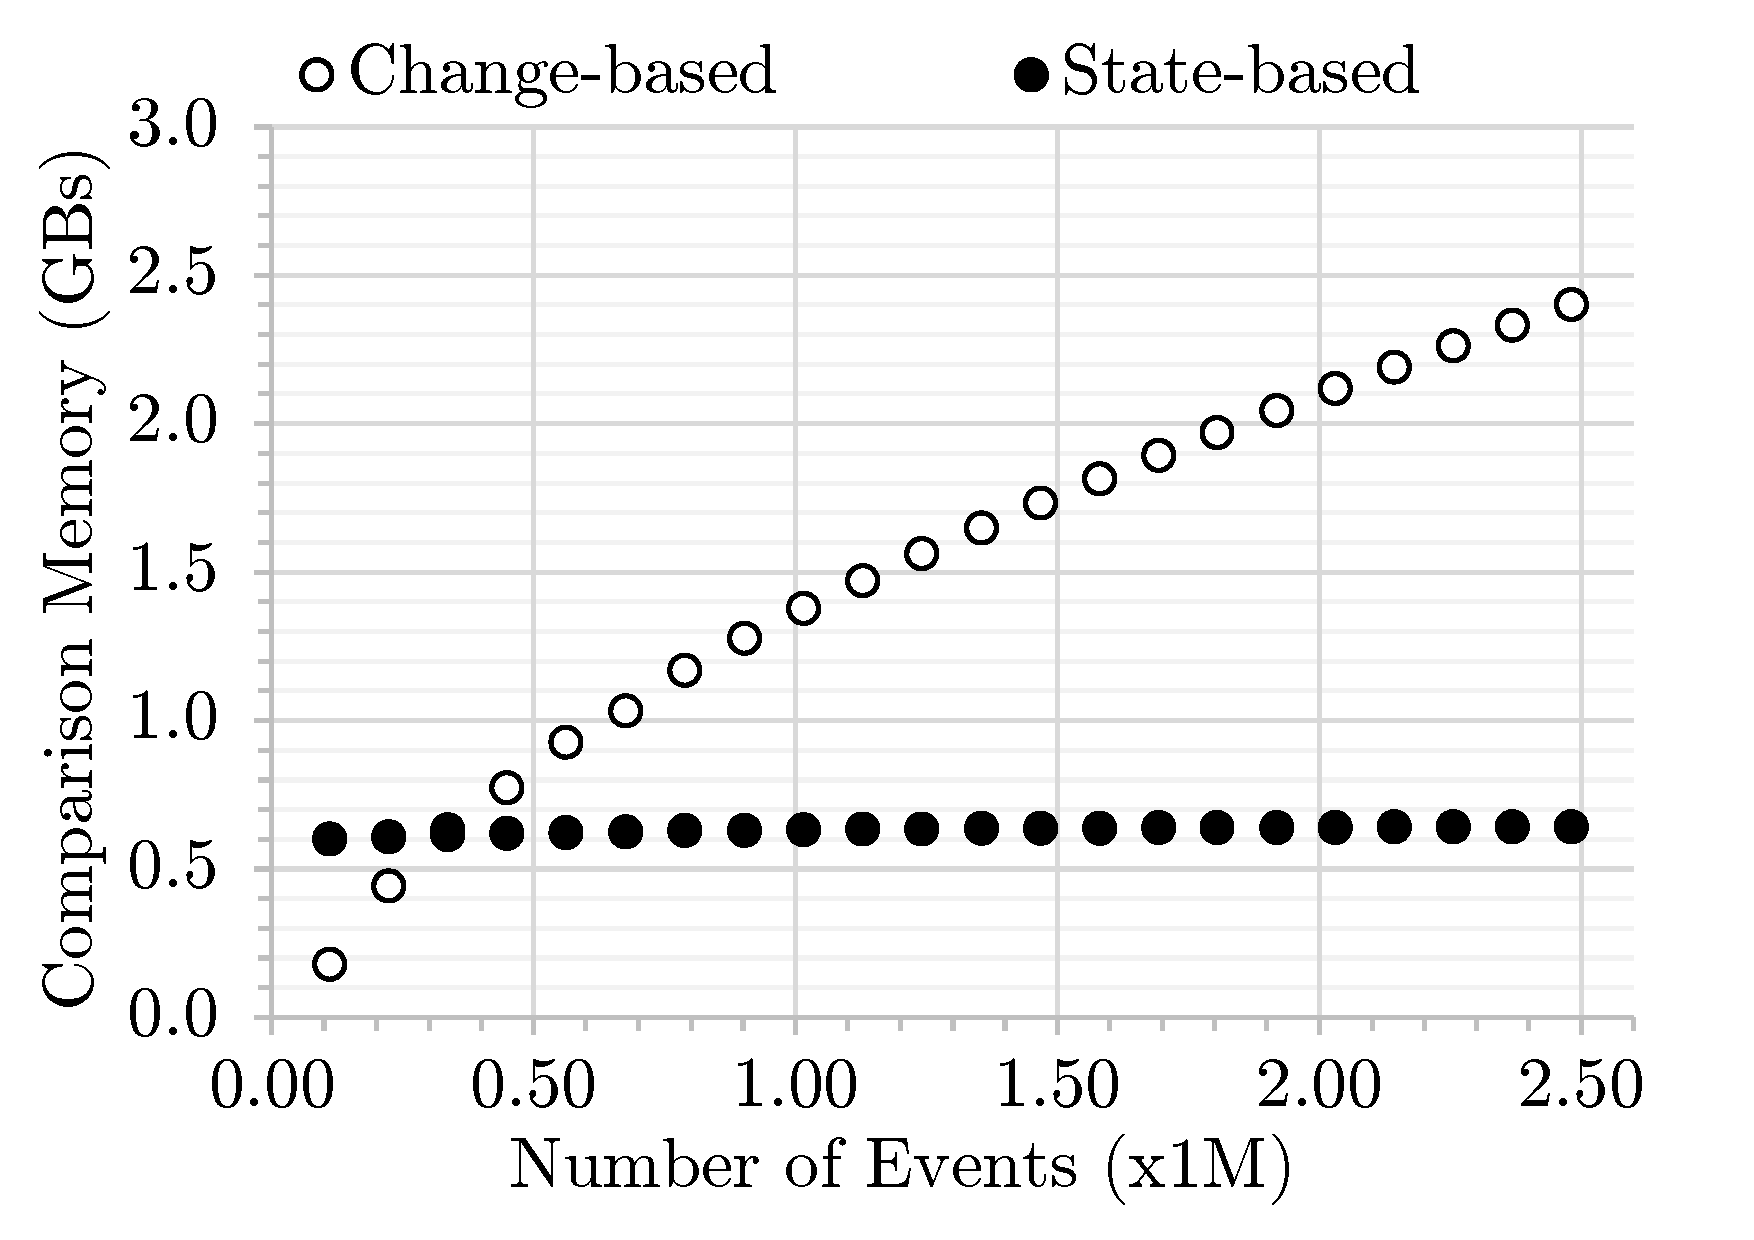
\includegraphics[width=\linewidth]{move-memory-events}
        \caption{move-only}
        \label{fig:move-memory-events}
    \end{subfigure}
    \hfill
    \begin{subfigure}[t]{0.495\linewidth}
        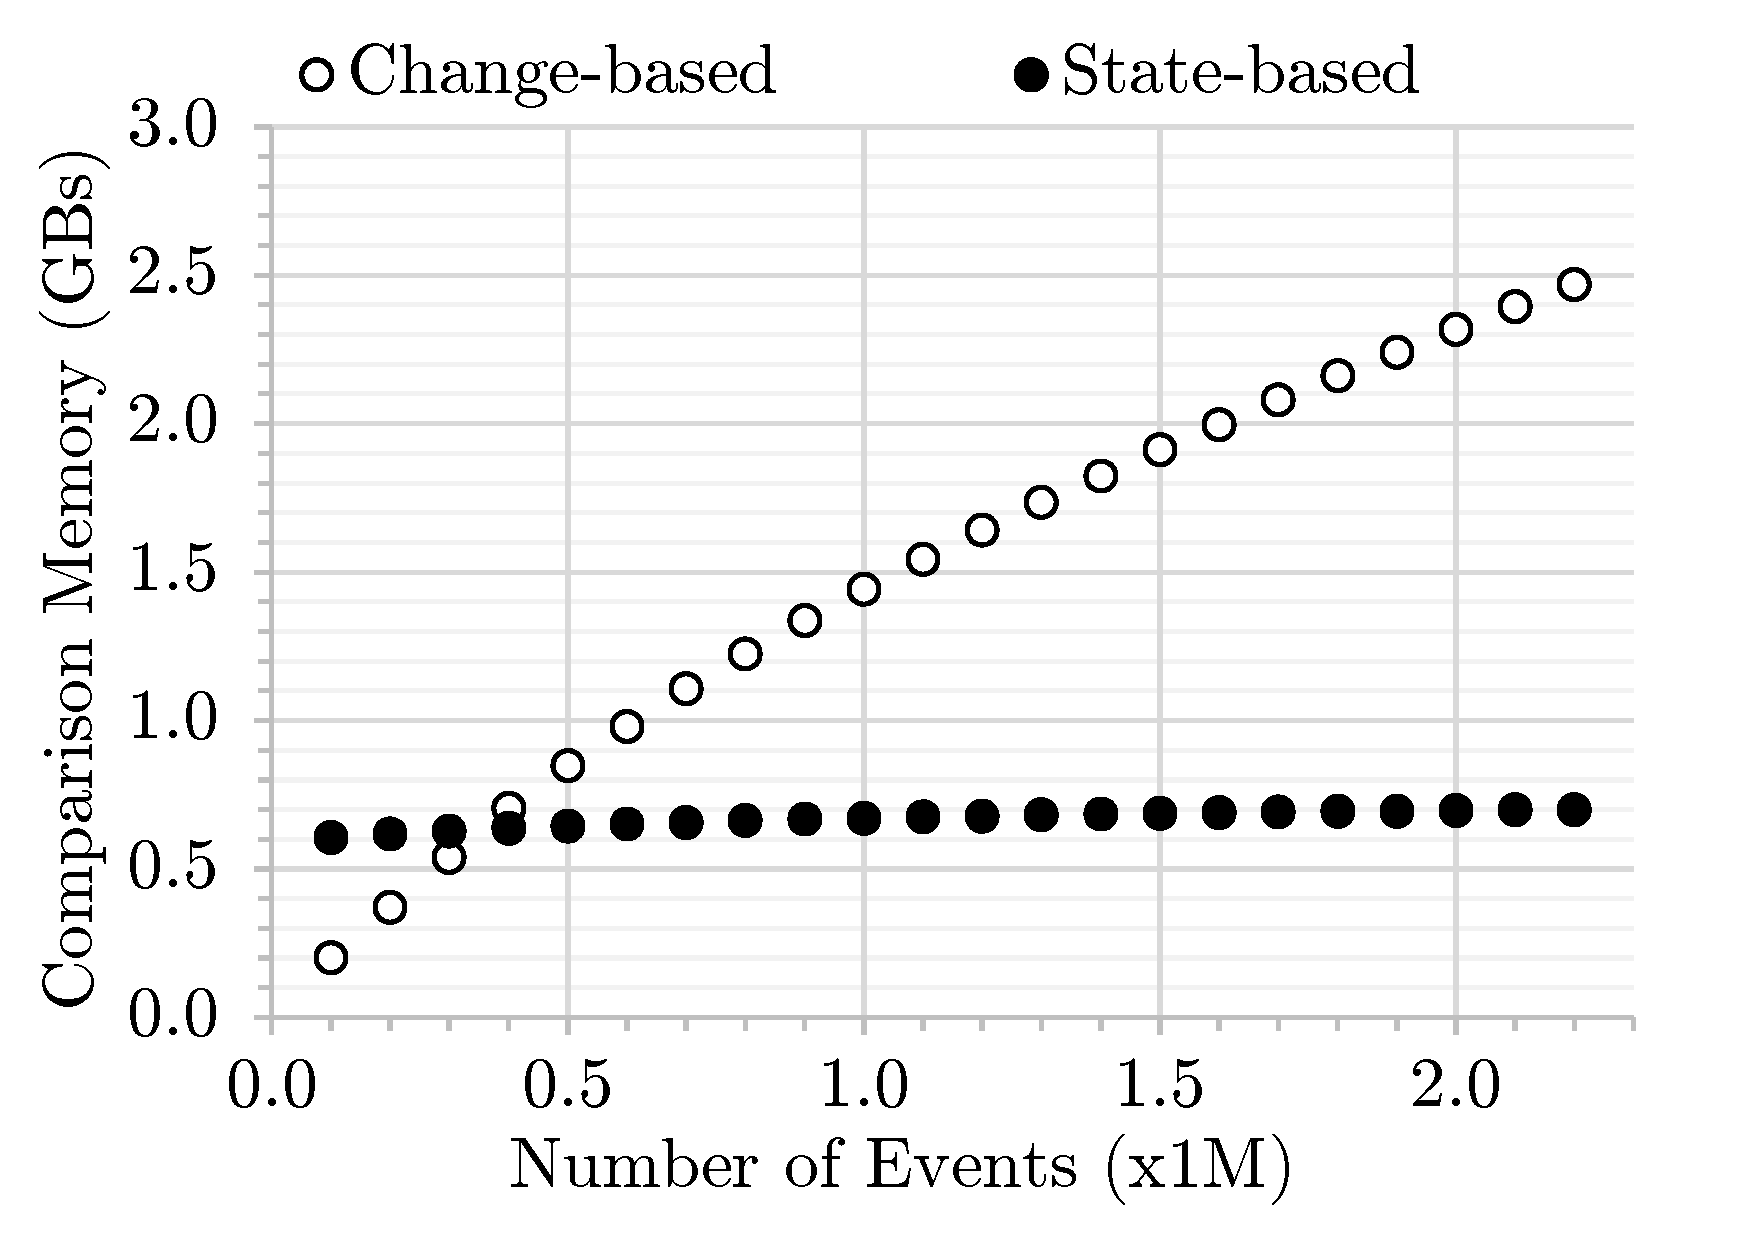
\includegraphics[width=\linewidth]{change-memory-events}
        \caption{change-only}
        \label{fig:change-memory-events}
    \end{subfigure}
    \caption{Memory footprint for homogeneous operations.}
    \label{fig:operation_memory_events}
\end{figure}

Figures \ref{fig:operation_time_events} and \ref{fig:operation_memory_events} exhibit the comparison time and memory footprint of models that have been modified using homogeneous operations -- \textsf{add}, \textsf{remove}, \textsf{move}, or \textsf{set} only. We can notice that in all figures change-based comparison outperforms its state-based counterpart particularly when the number of change events is small to moderate. If modification keeps continue, there is a point when the number of events is in great amount that the change-based comparison is slower than the state-based comparison. In our evaluation, it is when the number of events is greater than 4 million events (Fig. \ref{fig:add-time-events}). A slower change-based comparison -- if compared to state-based comparison -- also happens when the size of models is shrinking as depicted in Fig. \ref{fig:delete-memory-events} as the change-based comparison keeps still needs to load number of change events and construct its element tree. In terms of memory footprint, change-based comparison only performs better than state-based comparison when the number of change events is less than 0.3 millions as depicted in Fig. \ref{fig:operation_memory_events}.

Based on the findings, we argue that the change-based comparison approach works at its best for large models that have been modified in a moderate number of changes. Models that have been excessively modified and experience significant reduction on model size could impair the performance of change-based comparison as a great number of change records have to be read and loaded into memory. 

\subsection{Limitation and Validity}
\label{sec:limitation_and_Threat_to_validity}
The proposed change-based comparison comes with a limitation that it heavily relies on the use of identifiers to efficiently address modified elements. Applying change-based persistent to models that use URI fragments as element's identifiers faces a challenge in that an element's identifier changes when it is moved to another location in a model. The evaluation of the proposed change-based comparison is limited to the Java metamodel only. Thus, there is no guarantee it will always work on models with different metamodels. Although, we have tried to cover as much as common changes made in EMF models (e.g. performing \textsf{add}/\textsf{remove}/\textsf{set}/\textsf{move} operations on \textsf{single}/\textsf{multi}-\textsf{valued} features, \textsf{attribute}/\textsf{reference} features, or \textsf{containment}/\textsf{non}-\textsf{containment} references), the random modification made in the evaluation does not largely reflect the evolution of models in the real world. This is challenging as different domains can have their own patterns of model evolution -- different problems, metamodels, modellers, etc.

\section{Related Work}
\label{sec:related_work}
There are existing tools for model comparison. SiDiff \cite{Treude2007SiDiff} and DSMDiff \cite{lin2009dsmdiff} view models as graphs. They create matches and define differences between elements based on the similarity of their features. However, both are limited in flexibility to exploit the metamodel or particularities of a modelling language. EMF Compare \cite{emfcompare2018developer}, an established tool for model comparison and merging, addresses this by providing an extensible platform which users can define custom algorithms for matching, diffing, conflict detection, and merging. Flexibility is also offered by ECL (Epsilon Comparison Language) \cite{kolovos2009ecl}, a hybrid, rule-based language for model comparison, which allows users to specify algorithms to match elements of homogeneous/heterogeneous models. All these tools work at the structural level; they compare models based on the states of models.

CDO \cite{eclipse2019cdo} is a model repository with pluggable backends. Persisting its models in state-based format limits itself to gain the potential benefits of CBP, such as precise conflict detection and resolution. AMOR \cite{DBLP:conf/sfm/BroschKLSWW12}, a model versioning platform, also compares models in state-based. However, it also uses records of changes/operations of models to improve the precision of conflict detection and resolution. For example, multiple conflicts caused by a composite operation should be resolved as one package, not as an individual conflict, to ensure consistency of resolution. EMFStore \cite{koegel2010emfstore} is a version control system for EMF models that stores model versions as packages of operations. Since it works purely in operations without considering the states of models, every operation is treated as a new change. Thus, concurrent operations that change the same feature to the same value are treated as conflicting operations. Moreover, the drawback of using a dedicated versioning system, as in CDO and EMFStore, is restricting users to adopt common textual version control systems (e.g. Git, SVN) for model versioning.  

\section{Conclusions and Future Work}
\label{sec:conclusion_and_future_work}
In this paper, we have presented a novel approach to model comparison by exploiting the nature of change-based persistence which allows us to find differences between versions of a model by only comparing the last set of changes between the source and reference model.
Our evaluation results suggest that using this approach, we can produce model comparison that is faster than traditional, state-based model comparison.
However, the change-based comparison approach needs to load change events from a change-based persistence into main memory and thus may requires more memory than for state-based comparison. In our evaluation, this occurs when the number of change events exceeds 400,000.
Arguably, diff and merge operations are usually performed on smaller deltas than our evaluation.
The next challenge for future work is to identify strategies to merge models optimally and persist the merging in the change-based way. 

\backmatter

% \emph{NB: Please be sure to include DOIs (Digital Object Identifiers) for all cited articles, where available}

\bibliographystyle{alphaurl}
\bibliography{references}

%\abouttheauthors

\begin{acknowledgments}
This work was partly supported by through a scholarship managed by \emph{Lembaga Pengelola Dana Pendidikan Indonesia} (Indonesia Endowment Fund for Education).
\end{acknowledgments}

\end{document}
